% Narrative talk: every frame shows its first half, the next page adds the second half in place.
% Build: pdflatex talk.tex (twice).  Figures: figs/ (copied from manuscripts/notes/, figures/, manuscripts/extension/figs/).
\documentclass[aspectratio=169,10pt]{beamer}

% ---------------------------------------------------------------- talk metadata (edit these)
\newcommand{\talkauthor}{Arnav Kapoor}
\newcommand{\talkinstitute}{IISER Bhopal}
\newcommand{\talkevent}{Progress meeting}

% ---------------------------------------------------------------- theme
\usepackage[T1]{fontenc}
\usepackage{lmodern}
\usepackage{booktabs,tabularx,colortbl,xcolor,amsmath,amssymb}
\usepackage{tikz}
\usetikzlibrary{positioning,arrows.meta,shapes.misc,calc}

\definecolor{ibar}{HTML}{0B3C6E}
\definecolor{iaccent}{HTML}{2A78D6}
\definecolor{iorange}{HTML}{EB6834}
\definecolor{igreen}{HTML}{0F8A5F}
\definecolor{ired}{HTML}{C0392B}
\definecolor{ifoot}{HTML}{E9EEF4}
\definecolor{ink}{HTML}{1F1F1E}
\definecolor{muted}{HTML}{6B6A63}

\usefonttheme{professionalfonts}
\setbeamertemplate{navigation symbols}{}
\setbeamercovered{invisible}
\setbeamercolor{normal text}{fg=ink,bg=white}
\setbeamercolor{structure}{fg=ibar}
\setbeamercolor{alerted text}{fg=iorange}
\setbeamercolor{frametitle}{fg=white,bg=ibar}
\setbeamerfont{frametitle}{size=\large,series=\bfseries}
\setbeamercolor{block title}{fg=white,bg=ibar}
\setbeamercolor{block body}{bg=ifoot}
\setbeamercolor{block title alerted}{fg=white,bg=iorange}
\setbeamercolor{block body alerted}{bg=iorange!8}
\setbeamercolor{block title example}{fg=white,bg=igreen}
\setbeamercolor{block body example}{bg=igreen!8}
\setbeamertemplate{blocks}[rounded][shadow=false]
\setbeamertemplate{itemize item}{\color{iaccent}\raisebox{0.15ex}{\scriptsize$\blacksquare$}}
\setbeamertemplate{itemize subitem}{\color{muted}\textendash}
\setbeamertemplate{enumerate item}{\color{ibar}\bfseries\insertenumlabel.}

% title bar with the current part on the right
\setbeamertemplate{frametitle}{%
  \nointerlineskip
  \begin{beamercolorbox}[wd=\paperwidth,ht=2.6ex,dp=1.3ex,leftskip=1.2em,rightskip=1.2em]{frametitle}
    \usebeamerfont{frametitle}\insertframetitle\hfill{\normalfont\footnotesize\color{white!70!ibar}\insertsectionhead}
  \end{beamercolorbox}
  \vspace{-0.2ex}{\color{iaccent}\rule{\paperwidth}{1.2pt}}\vspace{0.2ex}}

\setbeamertemplate{footline}{%
  \leavevmode\hbox{\scriptsize%
  \begin{beamercolorbox}[wd=.30\paperwidth,ht=2.4ex,dp=1ex,leftskip=1em]{author in head/foot}%
    \color{white}\talkauthor\end{beamercolorbox}%
  \begin{beamercolorbox}[wd=.48\paperwidth,ht=2.4ex,dp=1ex,center]{title in head/foot}%
    \color{ink}\insertshorttitle\end{beamercolorbox}%
  \begin{beamercolorbox}[wd=.22\paperwidth,ht=2.4ex,dp=1ex,right,rightskip=1em]{date in head/foot}%
    \color{ink}\insertframenumber/\inserttotalframenumber\end{beamercolorbox}}}
\setbeamercolor{author in head/foot}{bg=ibar}
\setbeamercolor{title in head/foot}{bg=ifoot}
\setbeamercolor{date in head/foot}{bg=ifoot}

\newcommand{\good}[1]{\textcolor{igreen}{\textbf{#1}}}
\newcommand{\bad}[1]{\textcolor{ired}{\textbf{#1}}}
\newcommand{\qual}[1]{\textcolor{iorange}{\textbf{#1}}}
\newcommand{\src}[1]{\par\vfill\hfill{\tiny\color{muted}#1}}
\newcommand{\takeaway}[1]{\par\vfill{\setlength{\fboxsep}{5pt}\colorbox{ifoot}{\parbox{\dimexpr\linewidth-10pt}{\small\color{ibar}\textbf{Takeaway.} #1}}}}
\newcommand{\two}{\uncover<2->}   % second half of a slide (text only: tables are never split)

% part divider
\newcommand{\partslide}[3]{%
  \section{#2}
  {\setbeamertemplate{footline}{}
  \begin{frame}[plain]
    \begin{tikzpicture}[remember picture,overlay]
      \fill[ibar] (current page.south west) rectangle (current page.north east);
      \node[anchor=west,text=white!60!ibar,font=\Large\bfseries] at ([xshift=3em,yshift=2.2em]current page.west) {Part #1};
      \node[anchor=west,text=white,font=\huge\bfseries] at ([xshift=3em,yshift=-0.4em]current page.west) {#2};
      \node[anchor=north west,text=white!85!ibar,text width=0.8\paperwidth,font=\normalsize] at ([xshift=3em,yshift=-2.4em]current page.west) {#3};
    \end{tikzpicture}
  \end{frame}}}

\title[Circuit reduction: reproduction and extension]
      {Optimisation-driven quantum circuit reduction}
\author{\talkauthor}

\begin{document}

% ================================================================ title
{\setbeamertemplate{footline}{}
\begin{frame}[plain]
  \begin{tikzpicture}[remember picture,overlay]
    \fill[ibar] (current page.north west) rectangle ([yshift=-0.55\paperheight]current page.north east);
    \fill[iaccent] ([yshift=-0.55\paperheight]current page.north west) rectangle ([yshift=-0.565\paperheight]current page.north east);
    \node[anchor=north west,text=white,font=\small] at ([xshift=2em,yshift=-1.6em]current page.north west) {\talkevent};
    \node[anchor=south west,text=white,text width=0.88\paperwidth,align=left]
      at ([xshift=2em,yshift=0.50\paperheight]current page.south west)
      {{\LARGE\bfseries Optimisation-driven quantum circuit reduction}\\[0.6em]
       {\large Reproduction, exact Clifford ground truth,\\ and a general hardware-aware optimiser}};
    \node[anchor=north west,text width=0.8\paperwidth,align=left]
      at ([xshift=2em,yshift=0.40\paperheight]current page.south west)
      {{\large\bfseries \talkauthor}\\[0.3em]{\color{muted}\talkinstitute}\\[1.4em]
       {\footnotesize\color{muted}Study of B.~Rosenhahn, T.~J.~Osborne, C.~Hirche,
        \emph{Optimization driven quantum circuit reduction},\\ New J.\ Phys.\ \textbf{27}, 104509 (2025), arXiv:2502.14715}};
  \end{tikzpicture}
\end{frame}}

% ================================================================ storyline
\begin{frame}{The story in one slide}\small
  \begin{columns}[T]
    \begin{column}{0.48\textwidth}
      \textbf{What I was asked to do}
      \begin{itemize}\setlength{\itemsep}{0.15em}
        \item Understand the paper, re-run every figure and table.
        \item Find its weaknesses.
        \item Extend it.
      \end{itemize}
      \vspace{0.4em}
      \textbf{What I found}
      \begin{itemize}\setlength{\itemsep}{0.15em}
        \item It reproduces, but with qualifications.
        \item Every gate it uses is \textbf{Clifford}, so exact optima are computable.
        \item Against them, the method is \textbf{3--4.5\(\times\)} from optimal.
      \end{itemize}
    \end{column}
    \begin{column}{0.48\textwidth}
      \two{
      \textbf{What I built}
      \begin{itemize}\setlength{\itemsep}{0.15em}
        \item Theory: when local rewriting is globally optimal; parity; what random benchmarks measure.
        \item A \textbf{general optimiser}: no Clifford assumption, real native gates, connectivity, calibrated noise,
              exact / state-aware / approximate semantics.
      \end{itemize}
      \vspace{0.4em}
      \textbf{Where it stands}
      \begin{itemize}\setlength{\itemsep}{0.15em}
        \item Proven optimum on 35/40 of the paper's 3-qubit circuits.
        \item On top of Qiskit L3 on 58 real algorithms: never more 2q gates, \(-13\,\%\) gates on IBM Heron.
        \item Extension paper drafted (12 pages); every output verified.
      \end{itemize}}
    \end{column}
  \end{columns}
\end{frame}

\begin{frame}{Roadmap}
  \begin{columns}[T]
    \begin{column}{0.48\textwidth}
      \begin{enumerate}\setlength{\itemsep}{0.7em}
        \item \textbf{The paper}: database-driven local rewriting
        \item \textbf{Reproduction}: what holds, what needs qualifying
        \item \textbf{Ground truth}: every gate is Clifford \(\Rightarrow\) exact optima
        \item \textbf{Theory}: exactness, parity, mixing, lower bounds
      \end{enumerate}
    \end{column}
    \begin{column}{0.48\textwidth}
      \begin{enumerate}\setcounter{enumi}{4}\setlength{\itemsep}{0.7em}
        \item \textbf{A general optimiser}: no Clifford crutch, real hardware
        \item \textbf{Results}: paper benchmarks, standard suites, noisy simulation
        \item \textbf{Wrap-up}: lessons, caveats, critique, next steps
      \end{enumerate}
    \end{column}
  \end{columns}
\end{frame}

% ################################################################ PART I
\partslide{I}{The paper}{Rosenhahn, Osborne \& Hirche: shorten circuits by replacing short windows with shorter equivalents from a precomputed database.}

\begin{frame}{Why shorten circuits at all?}
  \begin{columns}[T]
    \begin{column}{0.47\textwidth}
      \begin{itemize}\setlength{\itemsep}{0.6em}
        \item On NISQ hardware every gate costs fidelity. Roughly,
              \[\Pr[\text{success}] \approx \prod_{\text{gates } g} \bigl(1-e(g)\bigr),\]
              with two-qubit errors \(\sim10^{-3}\)--\(10^{-2}\), 10--100\(\times\) single-qubit ones.
        \item Compiling to a device's \textbf{native alphabet} leaves redundancy:
              one textbook gate becomes several native ones, and neighbours stop cancelling.
        \item Goal: an equivalent circuit with fewer (or cheaper) native gates.
      \end{itemize}
    \end{column}
    \begin{column}{0.51\textwidth}
      \two{
      \centering
      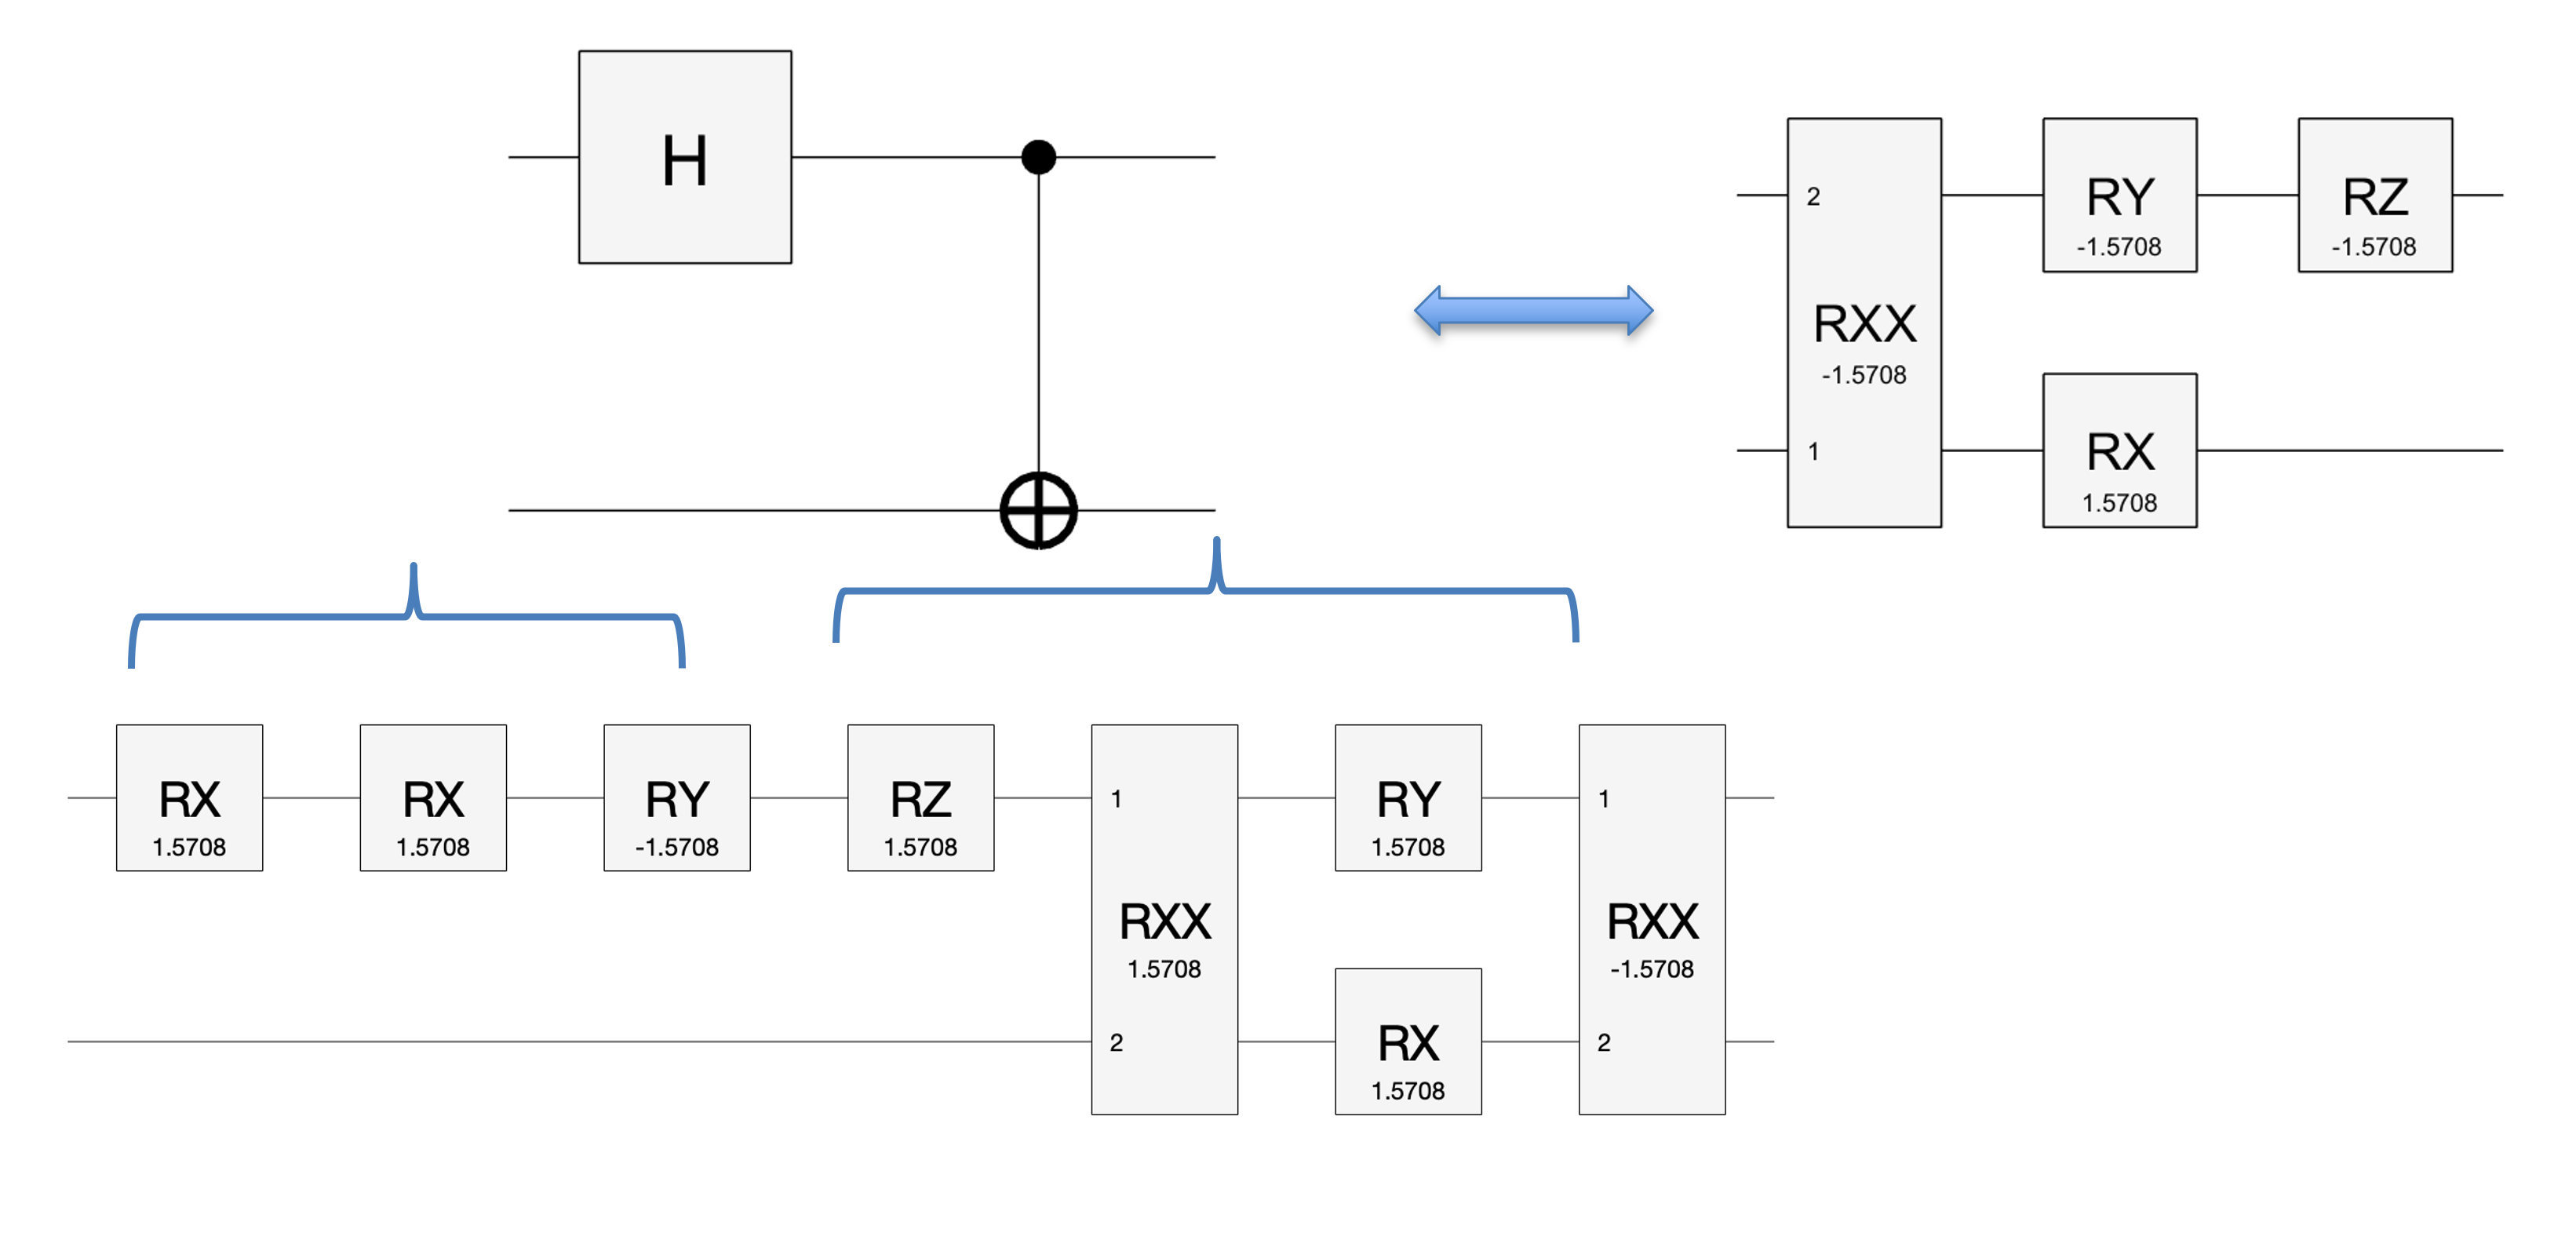
\includegraphics[width=\linewidth]{figs/Motivation1.png}\\[0.3em]
      {\scriptsize\color{muted}The paper's motivating example: H + CNOT compiled to the ion-trap alphabet (8 gates)
       and the shortest equivalent native word (4 gates). We confirmed by exhaustive search that no 3-gate version exists.}}
    \end{column}
  \end{columns}
  \src{Figure: arXiv:2502.14715, Fig.~1}
\end{frame}

\begin{frame}{Step 1: the compute graph, a database of shortest circuits}
  \begin{columns}[T]
    \begin{column}{0.47\textwidth}
      \begin{itemize}\setlength{\itemsep}{0.5em}
        \item Fix a \textbf{discrete alphabet} on 2--3 qubits:
          \begin{itemize}
            \item ion trap: \(R_{x},R_y,R_z(\pm\tfrac{\pi}{2})\), \(R_{XX}(\pm\tfrac{\pi}{2})\)
            \item IBM-style: \(R_x,R_z(\pm\tfrac{\pi}{2})\), CZ
          \end{itemize}
        \item Breadth-first search over words: each node is a unitary (up to global phase), stored with its
              \emph{shortest} word.
        \item Depth \(d\) = maximal word length enumerated.
      \end{itemize}
      \two{
      \vspace{0.4em}\centering\footnotesize
      \begin{tabular}{@{}lrrrrr@{}}
        \toprule
        depth & 1 & 2 & 3 & 4 & 5\\\midrule
        2q, 14 ops & 15 & 114 & 584 & 2,024 & 4,512\\
        3q, 24 ops & 25 & 337 & 3,215 & 23,622 & 137,572\\\bottomrule
      \end{tabular}\\[0.2em]
      {\scriptsize\color{muted}Table I node counts: our rebuild matches the paper exactly.}}
    \end{column}
    \begin{column}{0.51\textwidth}
      \centering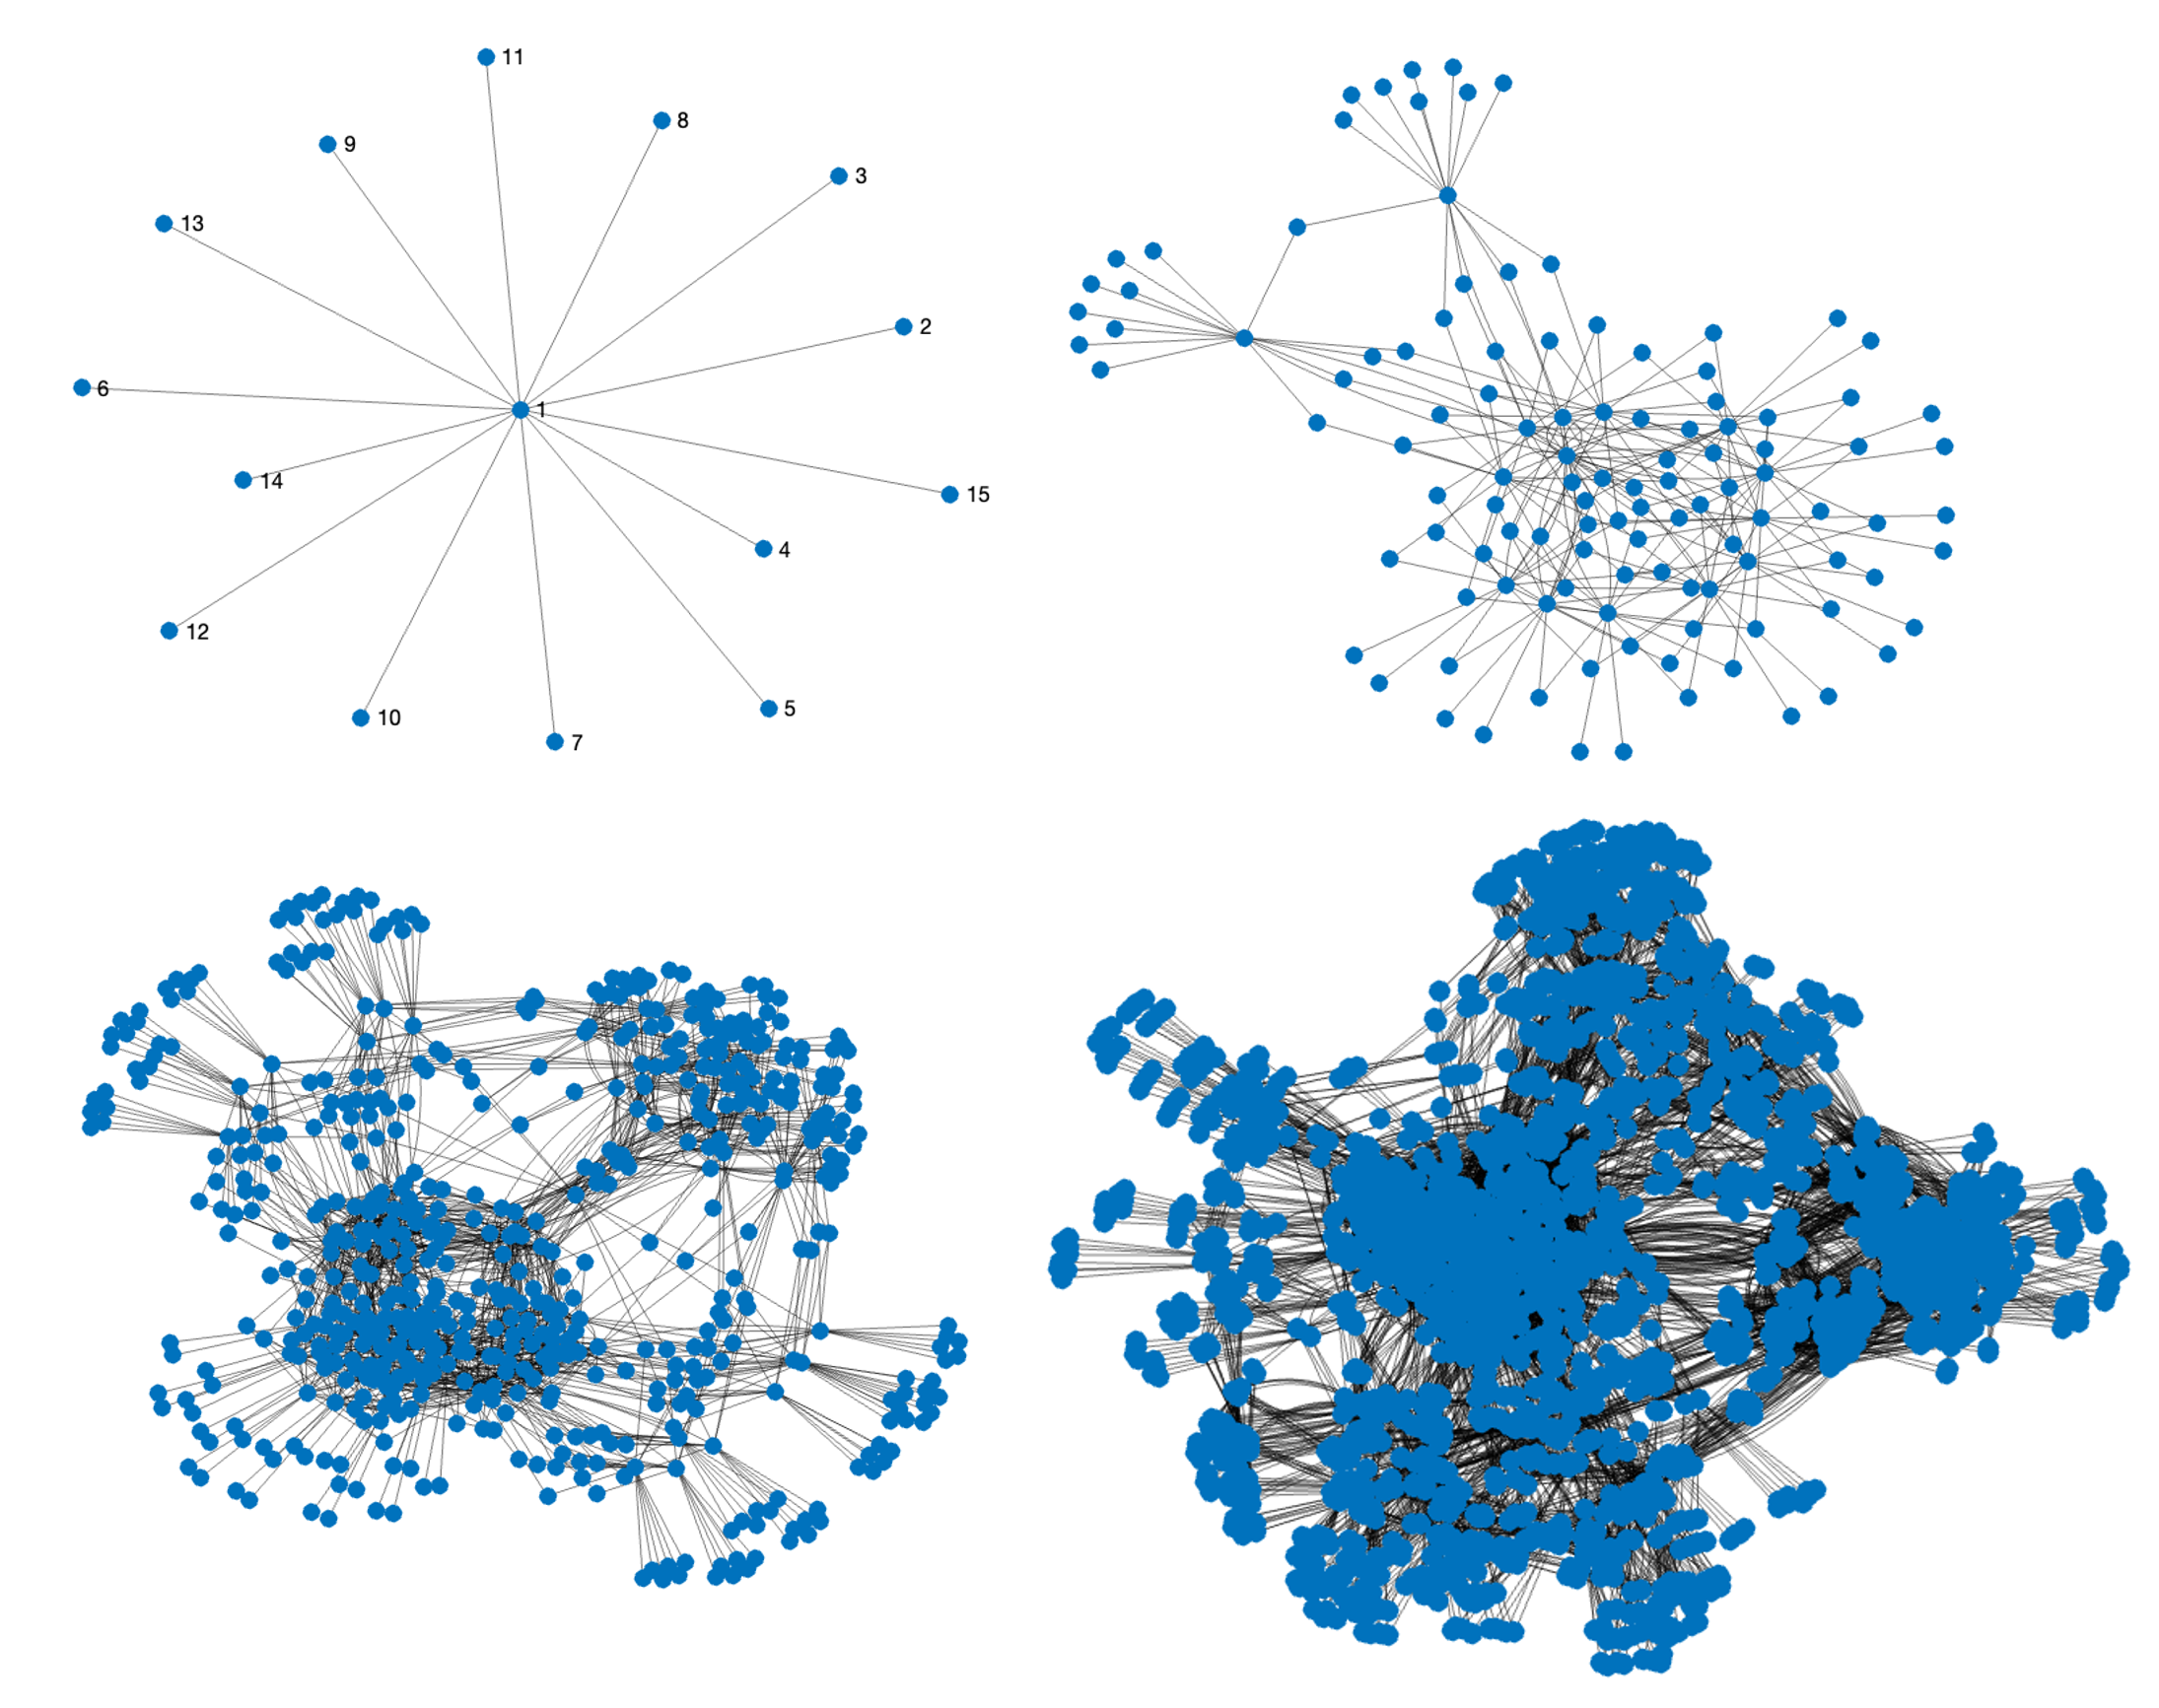
\includegraphics[width=0.9\linewidth]{figs/FullComputeGraphs2.png}\\[0.2em]
      {\scriptsize\color{muted}Compute graphs of growing depth (paper, Fig.~2).}
    \end{column}
  \end{columns}
\end{frame}

\begin{frame}{Step 2: slide a window, replace, repeat}
  \begin{columns}[T]
    \begin{column}{0.49\textwidth}
      \centering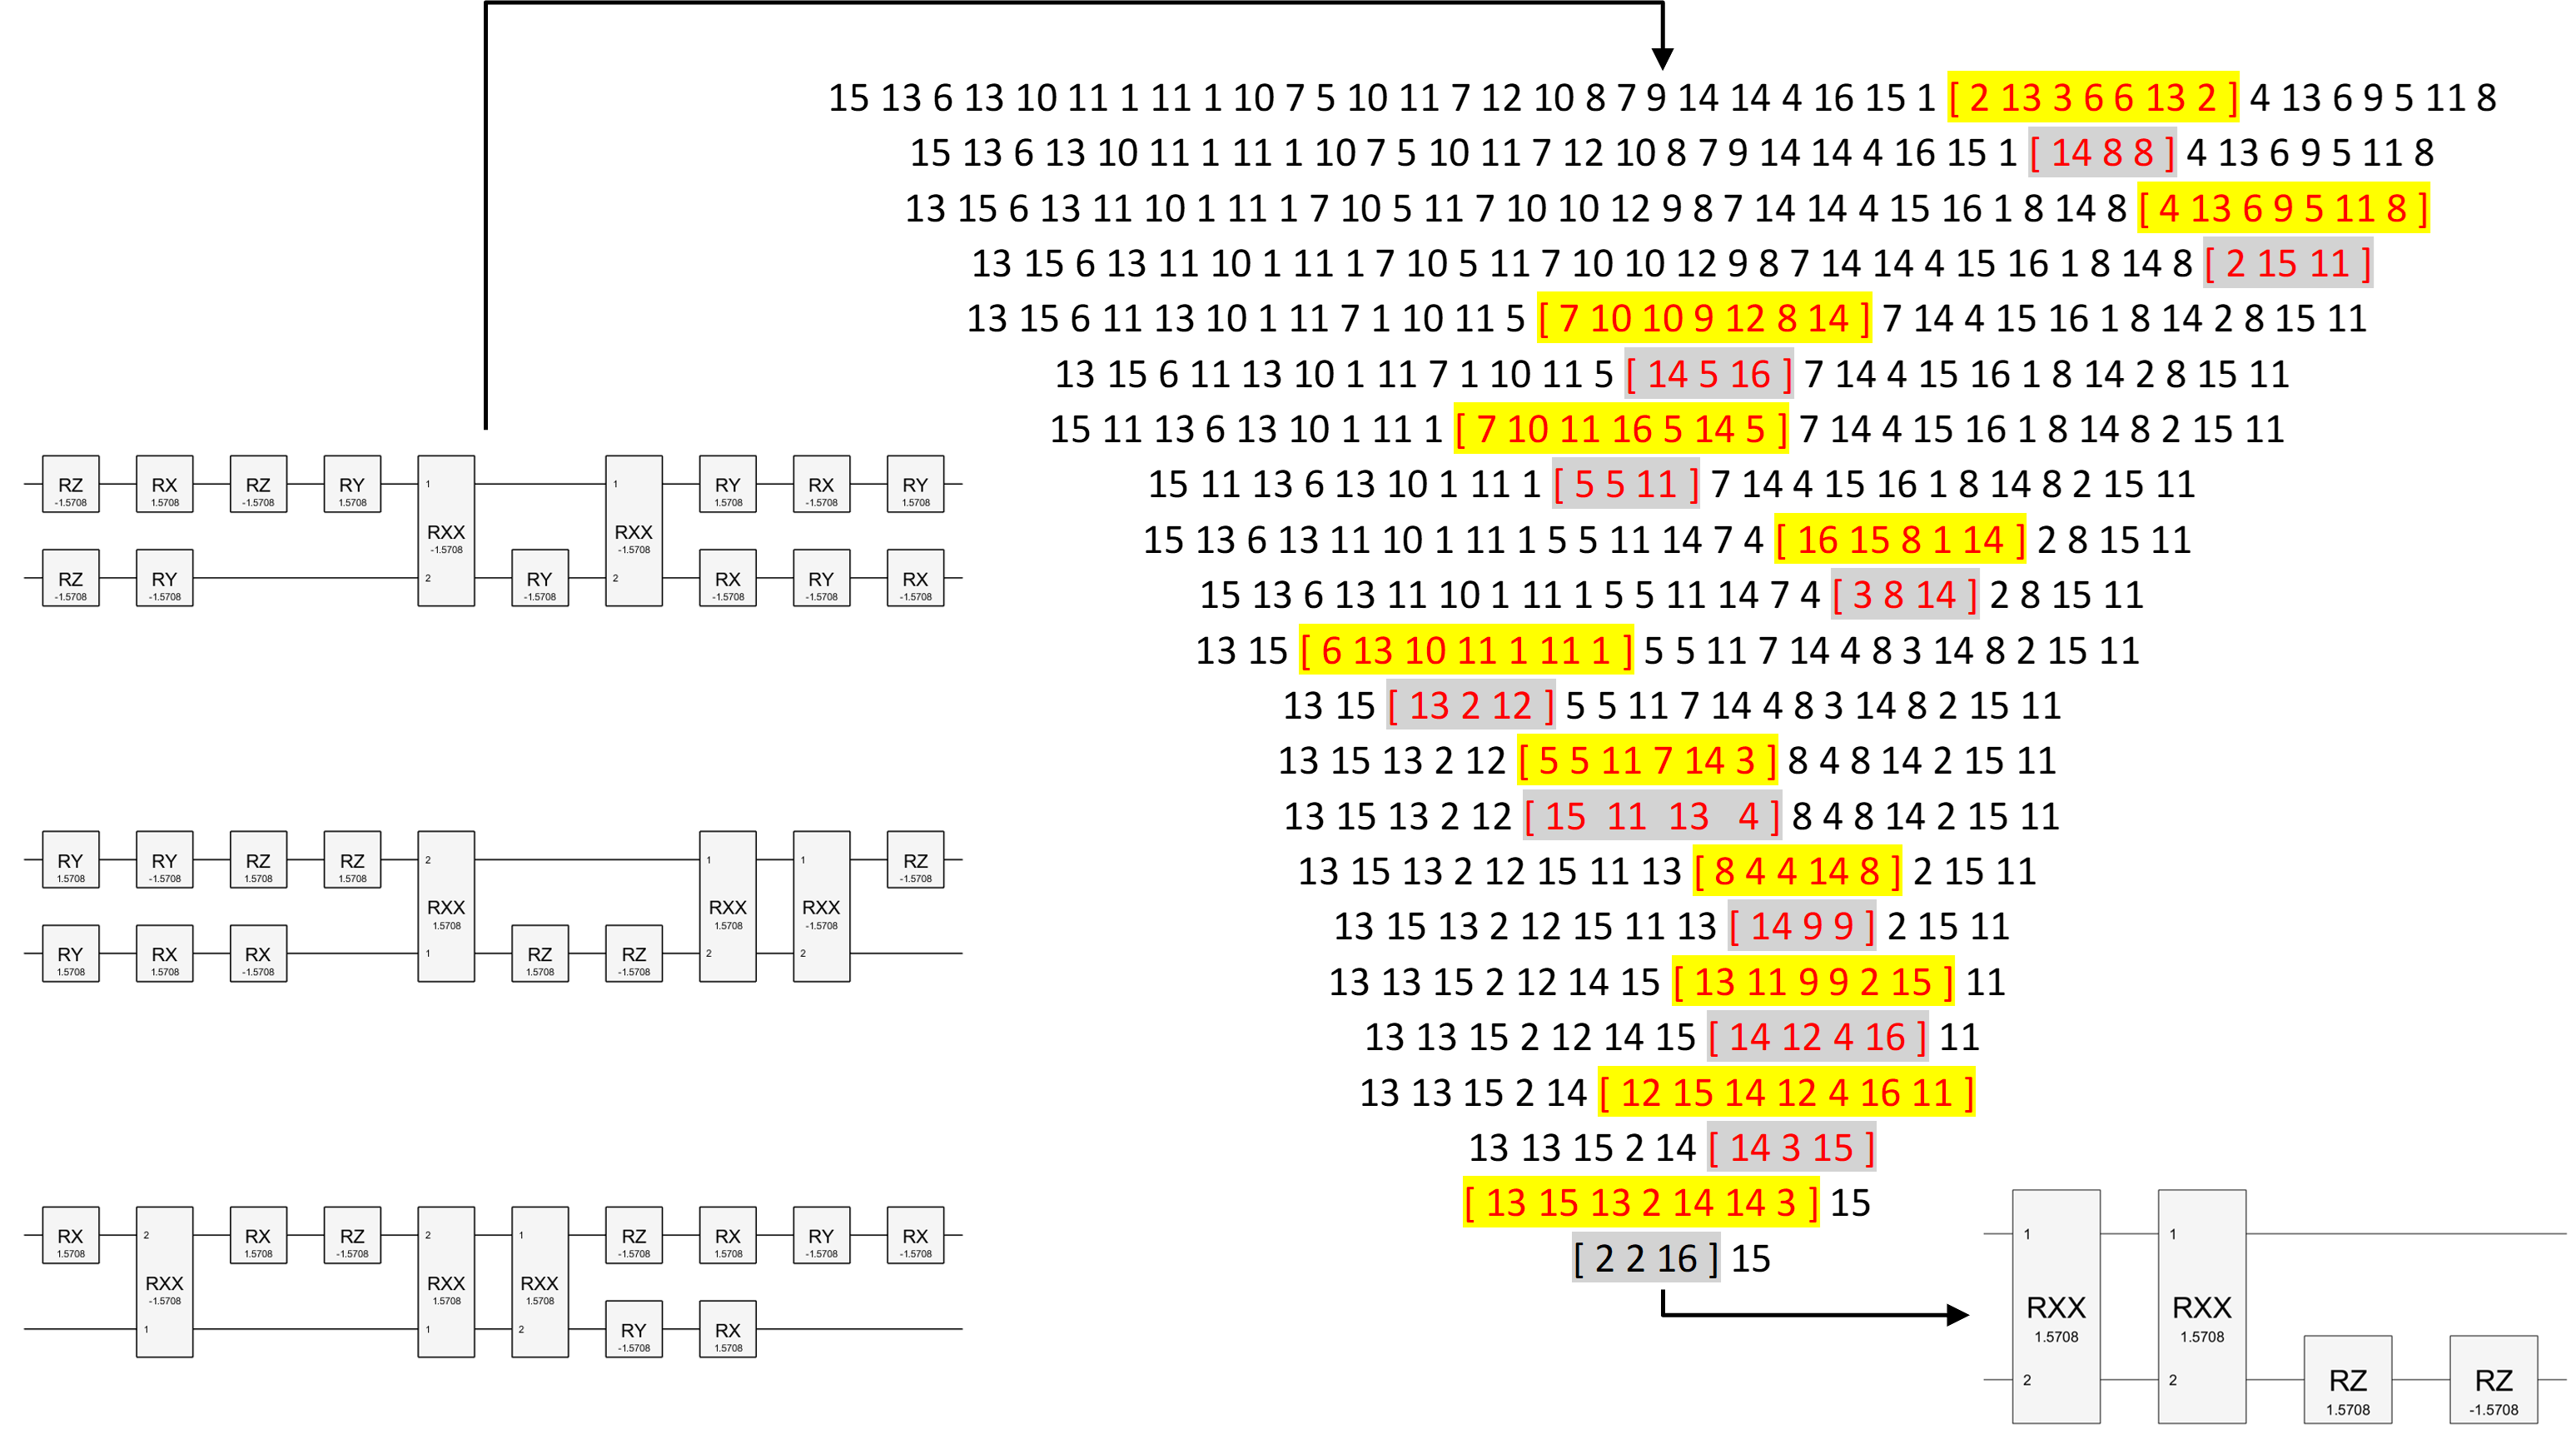
\includegraphics[width=0.85\linewidth]{figs/CodeReduceTokens.png}\\[0.2em]
      {\scriptsize\color{muted}Circuit as a word of tokens; windows are replaced by shorter database words (paper, Fig.~3).}
      \vspace{0.5em}
      \begin{itemize}\setlength{\itemsep}{0.3em}\small
        \item Pick a window of 2--8 gates on \(\le 3\) wires.
        \item Look its unitary up; if a shorter word exists, substitute it.
        \item Shuffle commuting gates to expose new windows; repeat until no progress.
      \end{itemize}
    \end{column}
    \begin{column}{0.49\textwidth}
      \two{
      \centering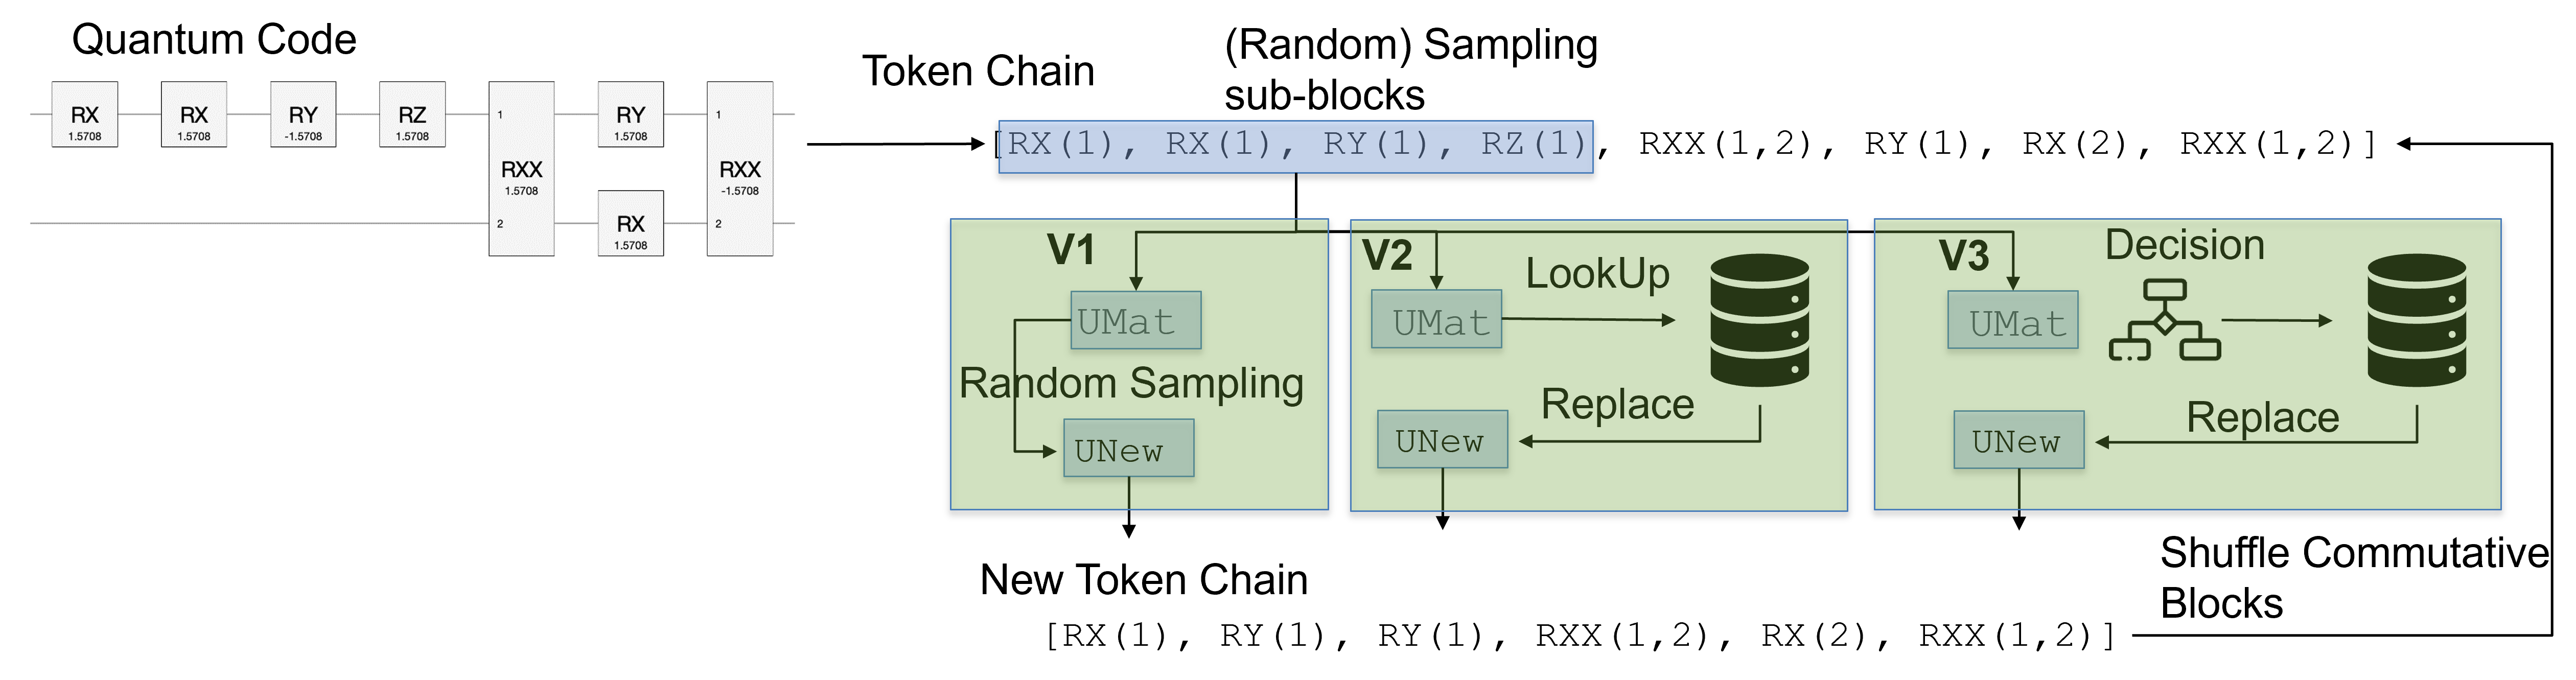
\includegraphics[width=\linewidth]{figs/optVariantsW.png}\\[0.3em]
      \begin{itemize}\setlength{\itemsep}{0.3em}\small
        \item \textbf{V1}: random sampling for a shorter equivalent word.
        \item \textbf{V2}: database lookup.
        \item \textbf{V3}: a random forest first predicts whether a window is reducible; only then look up.
      \end{itemize}}
    \end{column}
  \end{columns}
  \src{Figures: arXiv:2502.14715, Figs.~3 and 6}
\end{frame}

\begin{frame}{Step 3: scaling up, and what the paper claims}
  \begin{columns}[T]
    \begin{column}{0.47\textwidth}
      \centering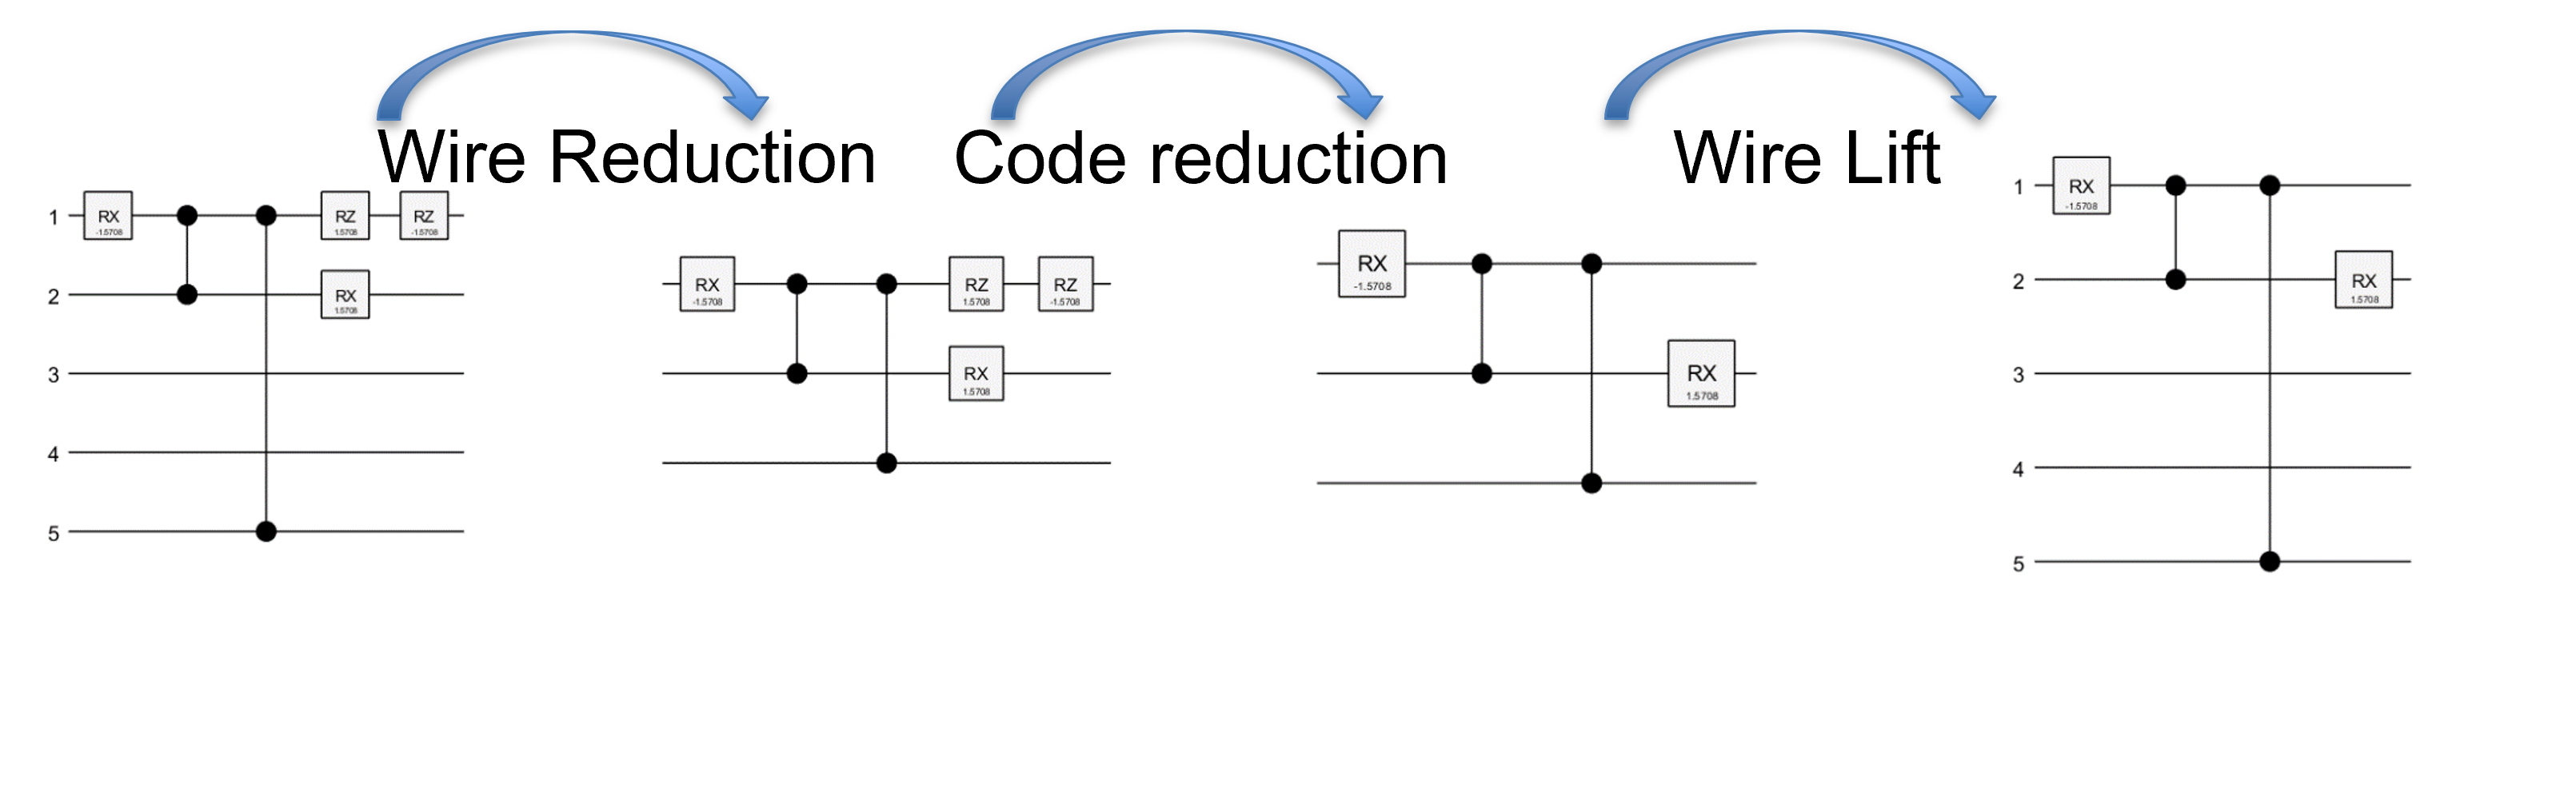
\includegraphics[width=\linewidth]{figs/ScalableOpt2.png}\\[0.2em]
      {\scriptsize\color{muted}Wire reduction / code reduction / wire lift: a 3-qubit database is applied inside an \(n\)-qubit circuit.}
    \end{column}
    \begin{column}{0.51\textwidth}
      \two{
      \textbf{Claims}\\[0.3em]
      \footnotesize\renewcommand{\arraystretch}{1.2}
      \resizebox{\linewidth}{!}{\begin{tabular}{@{}lrr@{}}
        \toprule
        benchmark (random native circuits) & paper & Qiskit (theirs)\\\midrule
        T.~III: ion, 3q, 300 gates & 45 & 176\\
        T.~IV: IBM-style, 3q, 300 gates & 72 & 153\\
        T.~V: IBM-style, 15q, 500 gates & 293 & 313\\
        journal: 4q, 300 gates (ion / IBM) & 111 / 107 & --\\
        T.~II time (s): V1 / V2 / V3 & \multicolumn{2}{l}{199 / 55 / 38}\\\bottomrule
      \end{tabular}}
      \vspace{0.6em}
      \begin{itemize}\small
        \item Fig.~9: reduced circuits give better results on IBM Brisbane and Kyiv.
      \end{itemize}}
    \end{column}
  \end{columns}
  \takeaway{A clean, gate-set-agnostic idea, evaluated against Qiskit only, on random words over a discrete alphabet.}
\end{frame}

% ################################################################ PART II
\partslide{II}{Reproduction}{Re-running every figure and table with a Python port of the authors' own MATLAB code.}

\begin{frame}{What I started from, and what I built}
  \begin{columns}[T]
    \begin{column}{0.48\textwidth}
      \textbf{Inputs}
      \begin{itemize}\setlength{\itemsep}{0.4em}
        \item arXiv PDF + LaTeX source, journal (NJP) PDF.
        \item Official code \texttt{QCOptimDemo.zip}: linked only in the journal's ref.~[38]; \textbf{V2 only}, MATLAB.
        \item Unspecified in the paper: database for Tables III--V, Table II protocol, forest details, transpiler level, Qiskit version.
      \end{itemize}
    \end{column}
    \begin{column}{0.48\textwidth}
      \two{
      \textbf{Built}
      \begin{itemize}\setlength{\itemsep}{0.4em}
        \item \texttt{qcr/}: line-by-line Python port (graph builder, V1/V2/V3, wire reduction), with tests.
        \item An independent exact engine (Clifford tableaux) as a cross-check.
        \item Every output checked equivalent to its input (unitary error \(\sim10^{-12}\)).
        \item Scripts + raw results for each table and figure; reproduction report (PDF).
      \end{itemize}}
    \end{column}
  \end{columns}
\end{frame}

\begin{frame}{Verdict at a glance}
  \renewcommand{\arraystretch}{1.3}\small
  \begin{tabularx}{\textwidth}{@{}p{0.28\textwidth}p{0.11\textwidth}X@{}}
    \toprule
    \textbf{Claim} & \textbf{Status} & \textbf{Detail}\\
    \midrule
    Table I (compute graphs) & \good{exact} & identical node and edge counts\\
    Figs.~1, 4, 5 (examples) & \good{yes} & same end points; Fig.~4 needs a different gate pool (parity, Part IV)\\
        Tables III/IV, journal 4q & \qual{qualified} & only with the 24-operator, depth-5 database (unstated)\\
    Table II: V1 \(>\) V2 \(>\) V3 & \qual{qualified} & V3 wins only with a tuned forest threshold\\
    Table V (15 qubits) & \bad{no longer} & ties a current Qiskit (2.5)\\
    Fig.~9 (hardware) & \qual{qualified} & real at Qiskit levels 0/1, disappears at level 3\\
    \bottomrule
  \end{tabularx}
  \two{\takeaway{The headline claim (beats Qiskit on few-qubit random circuits) holds; the details around it need qualifying.}}
\end{frame}

\begin{frame}{Table II: V1 vs.\ V2 vs.\ V3}
  \begin{columns}[T]
    \begin{column}{0.50\textwidth}
      \footnotesize\renewcommand{\arraystretch}{1.2}
      \resizebox{\linewidth}{!}{\begin{tabular}{@{}lrrrr@{}}
        \toprule
        variant & mean (s) & median (s) & reached & lookups\\\midrule
        V1 random sampling & 254.0 & 134.2 & 73 & 51,350\\
        V2 database & 46.4 & 6.5 & 96 & 7,904\\
        V3 forest, \(t=0.5\) & 171.8 & 16.9 & 79 & 915\\
        V3 forest, \(t=0.2\) & 33.7 & 5.3 & 98 & 1,216\\\bottomrule
      \end{tabular}}\\[0.3em]
      {\scriptsize\color{muted}100 random 5-qubit ion circuits, length 100 \(\to\) target 60, cap 600\,s. Paper: 199 / 55 / 38\,s.}
      \vspace{0.6em}
      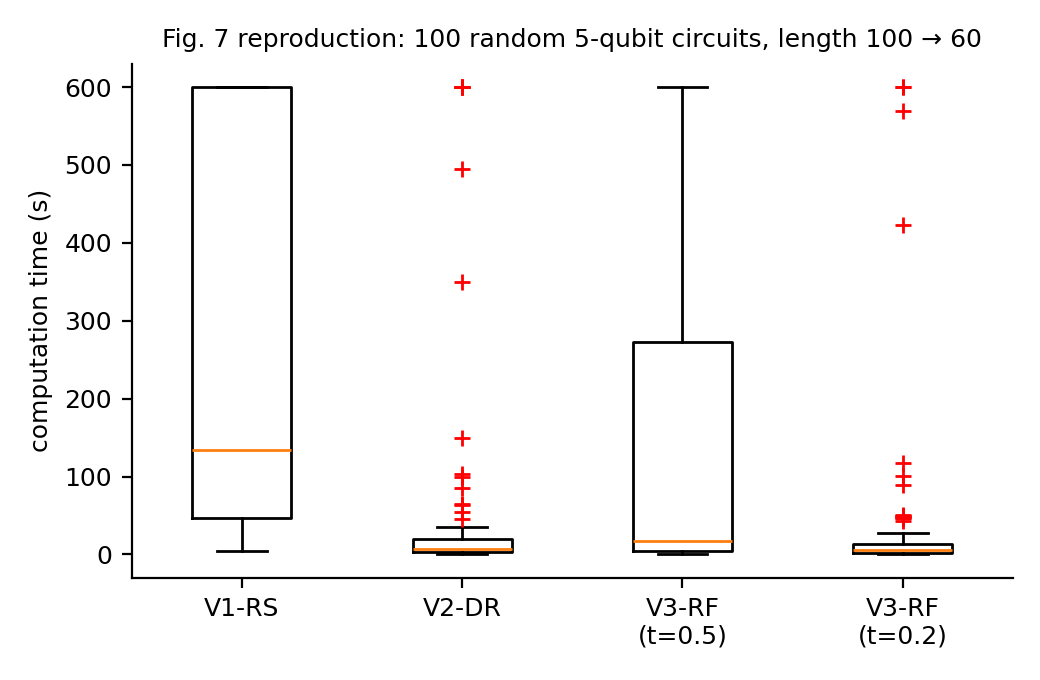
\includegraphics[width=0.85\linewidth]{figs/repro_boxplot.png}
    \end{column}
    \begin{column}{0.48\textwidth}
      \two{
      \begin{itemize}\setlength{\itemsep}{0.6em}
        \item V1 \(\gg\) V2 holds: the database is a real speed-up.
        \item V3 depends entirely on the forest's \textbf{recall}: on held-out windows it flags only
              \textbf{30\,\%} of reducible ones at the default threshold 0.5 (92\,\% at 0.2).
        \item At 0.5 it discards most reductions and is \emph{slower} than V2. The paper reports neither features,
              forest size, threshold nor accuracy.
      \end{itemize}
      \takeaway{The ``learning'' variant only helps after tuning a threshold the paper does not mention, and it saves time on a lookup that need not be slow.}}
    \end{column}
  \end{columns}
\end{frame}

\begin{frame}{Tables III--V and the journal statistics: comparison with Qiskit}
  \centering\footnotesize\renewcommand{\arraystretch}{1.2}
  \resizebox{\textwidth}{!}{\begin{tabular}{@{}lrrrrr@{}}
    \toprule
    benchmark & input & Qiskit (paper) & Qiskit 2.5 L3 & paper & our faithful port\\\midrule
    T.~III ion, 3q (20 circuits) & 300 & 176 & 127.2 & 45 & \good{47.1}\\
    T.~IV IBM-style, 3q (20) & 300 & 153 & 104.0 & 72 & \good{36.8}\\
    journal ion, 4q (30) & 300 & -- & 164.9 & 111 & \good{78.8}\\
    journal IBM-style, 4q (30) & 300 & -- & 140.9 & 107 & \good{76.0}\\
    T.~V IBM-style, 15q (10) & 500 & 313 & 332.1 & 293 & \bad{335.9}\\\bottomrule
  \end{tabular}}
  \vspace{0.8em}
  \two{
  \begin{columns}[T]
    \begin{column}{0.48\textwidth}
      \begin{itemize}\setlength{\itemsep}{0.3em}\small
        \item Few qubits: the method clearly beats Qiskit, as claimed; our port is even better than published.
        \item But only with the larger database (24 operators, depth 5), which the paper does not state.
      \end{itemize}
    \end{column}
    \begin{column}{0.48\textwidth}
      \begin{itemize}\setlength{\itemsep}{0.3em}\small
        \item Qiskit 2.5 is much stronger than the paper's Qiskit at 3 qubits (127 vs.\ 176; 104 vs.\ 153).
        \item 15 qubits: our port reaches 335.9 (paper 293) and only ties Qiskit L3 (332.1, same CZ count). Random 15-qubit gate pairs rarely share wires, so 3-wire windows find little that Qiskit misses.
      \end{itemize}
    \end{column}
  \end{columns}}
\end{frame}

\begin{frame}{Fig.~9: the hardware experiment, in a noisy simulator}
  \begin{columns}[T]
    \begin{column}{0.52\textwidth}
      \centering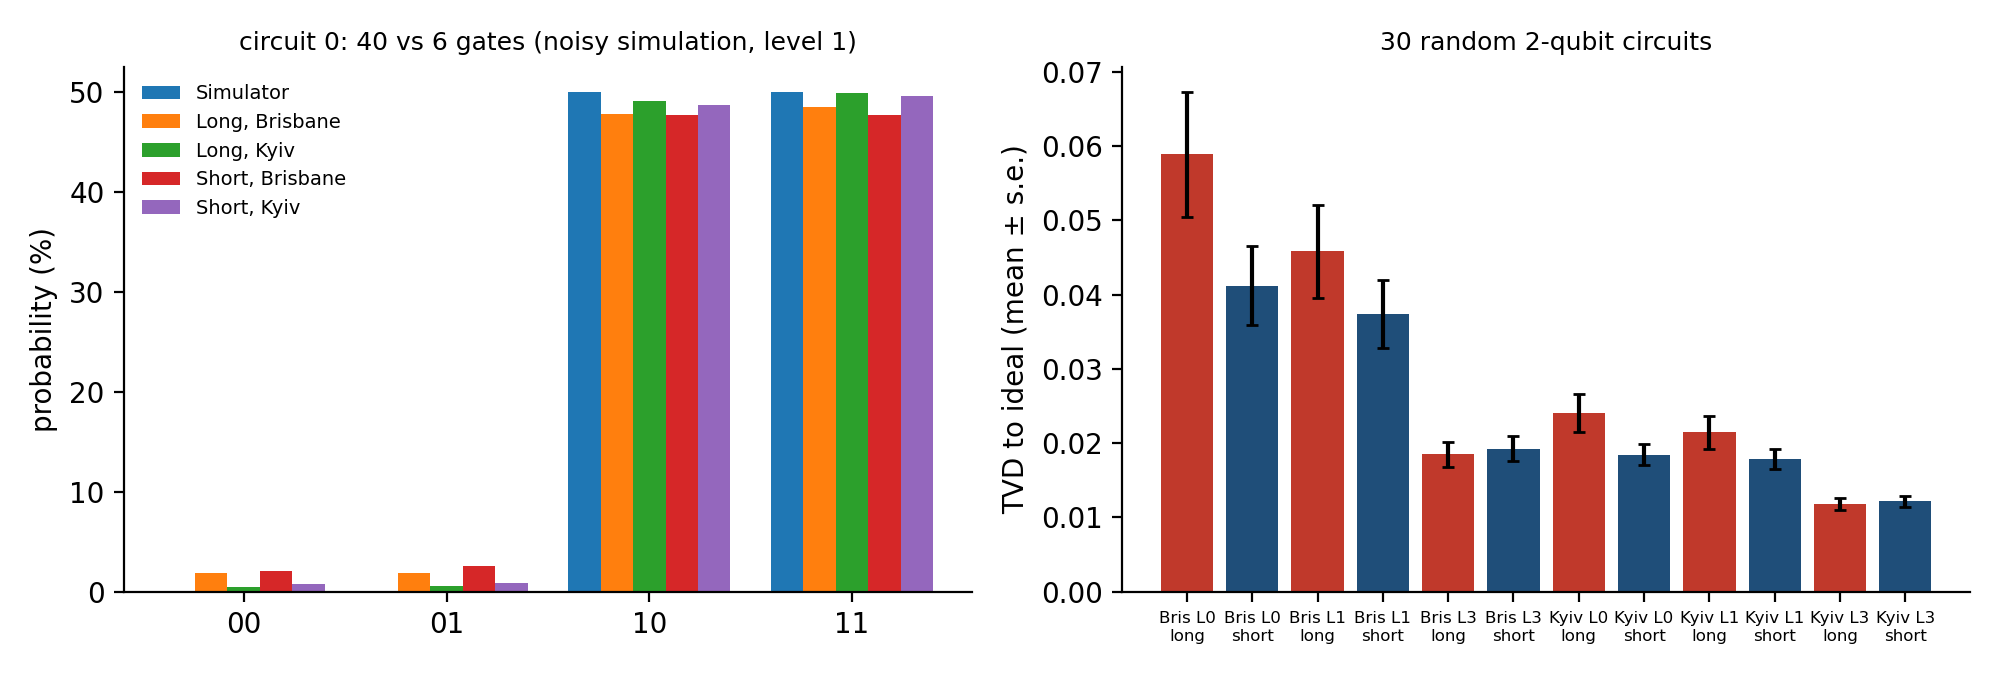
\includegraphics[width=\linewidth]{figs/repro_hardware.png}\\[0.3em]
      \footnotesize\renewcommand{\arraystretch}{1.15}
      \resizebox{\linewidth}{!}{\begin{tabular}{@{}lccc@{}}
        \toprule
        TVD to ideal (30 circuits) & level 0 & level 1 & level 3\\\midrule
        Brisbane: long \(\to\) reduced & 0.059 \(\to\) 0.041 & 0.046 \(\to\) 0.037 & 0.018 vs.\ 0.019\\
        Kyiv: long \(\to\) reduced & 0.024 \(\to\) 0.018 & 0.021 \(\to\) 0.018 & 0.012 vs.\ 0.012\\\bottomrule
      \end{tabular}}
    \end{column}
    \begin{column}{0.46\textwidth}
      \two{
      \begin{itemize}\setlength{\itemsep}{0.5em}
        \item Levels 0/1: the reduced circuit is closer to ideal (22/30 and 20/30 circuits), as in the paper.
        \item Level 3: Qiskit re-synthesises every 2-qubit block, both versions compile to \(\approx1.1\) CZ, the effect \textbf{vanishes}.
        \item Plain Qiskit L3 on the \emph{long} circuit beats the reduced circuit at level 1 (0.018 vs.\ 0.037).
        \item Paper: one circuit, one run per chip, no error bars, transpiler level not stated.
      \end{itemize}}
    \end{column}
  \end{columns}
\end{frame}

\begin{frame}{Bugs and unstated choices found along the way}
  \begin{columns}[T]
    \begin{column}{0.48\textwidth}
      \textbf{In the released code}
      \begin{enumerate}\setlength{\itemsep}{0.4em}\small
        \item \texttt{simplereduce} never tests the last adjacent pair, and skips the pair after a deletion: the final circuit in the paper's Fig.~4
              still contains an inverse pair (true optimum 2, shown 4).
        \item The database excludes the identity, so identity blocks are never deleted by lookup.
        \item Three tolerances: \(10^{-5}\) (paper), \(10^{-3}\) (optimiser), \(10^{-4}\) (graph builder).
      \end{enumerate}
    \end{column}
    \begin{column}{0.48\textwidth}
      \two{
      \textbf{In the paper}
      \begin{enumerate}\setcounter{enumi}{3}\setlength{\itemsep}{0.4em}\small
        \item Gate pool: Table I implies 14/24 operators, the demo uses 13/21.
        \item Database for Tables III--V unstated; only the larger one reproduces Table III.
        \item Table II: qubit count and target length unstated; forest unspecified.
        \item Hardware: text says RX, RY, CX; tables say RX, RZ, CZ; transpiler level and shots unstated.
      \end{enumerate}}
    \end{column}
  \end{columns}
\end{frame}

% ################################################################ PART III
\partslide{III}{Exact ground truth}{The observation the paper misses: every gate it uses is Clifford, so the search space is a finite group we can enumerate completely.}

\begin{frame}{Key observation: every gate in the paper is Clifford}
  \begin{columns}[T]
    \begin{column}{0.48\textwidth}
      \begin{itemize}\setlength{\itemsep}{0.5em}
        \item \(\pm\tfrac{\pi}{2}\) rotations, \(R_{XX}(\pm\tfrac{\pi}{2})\) and CZ map Paulis to Paulis.
        \item So every circuit is an element of the finite \textbf{Clifford group} \(\mathcal C_n\) (mod phase), of order
              \[2^{n^2+2n}\prod_{j=1}^n (4^j-1)\]
              \(n=1\): 24, \(n=2\): 11,520, \(n=3\): \textbf{92,897,280}.
        \item The paper's ``compute graph'' is a ball in the \textbf{Cayley graph} of this group.
      \end{itemize}
    \end{column}
    \begin{column}{0.50\textwidth}
      \centering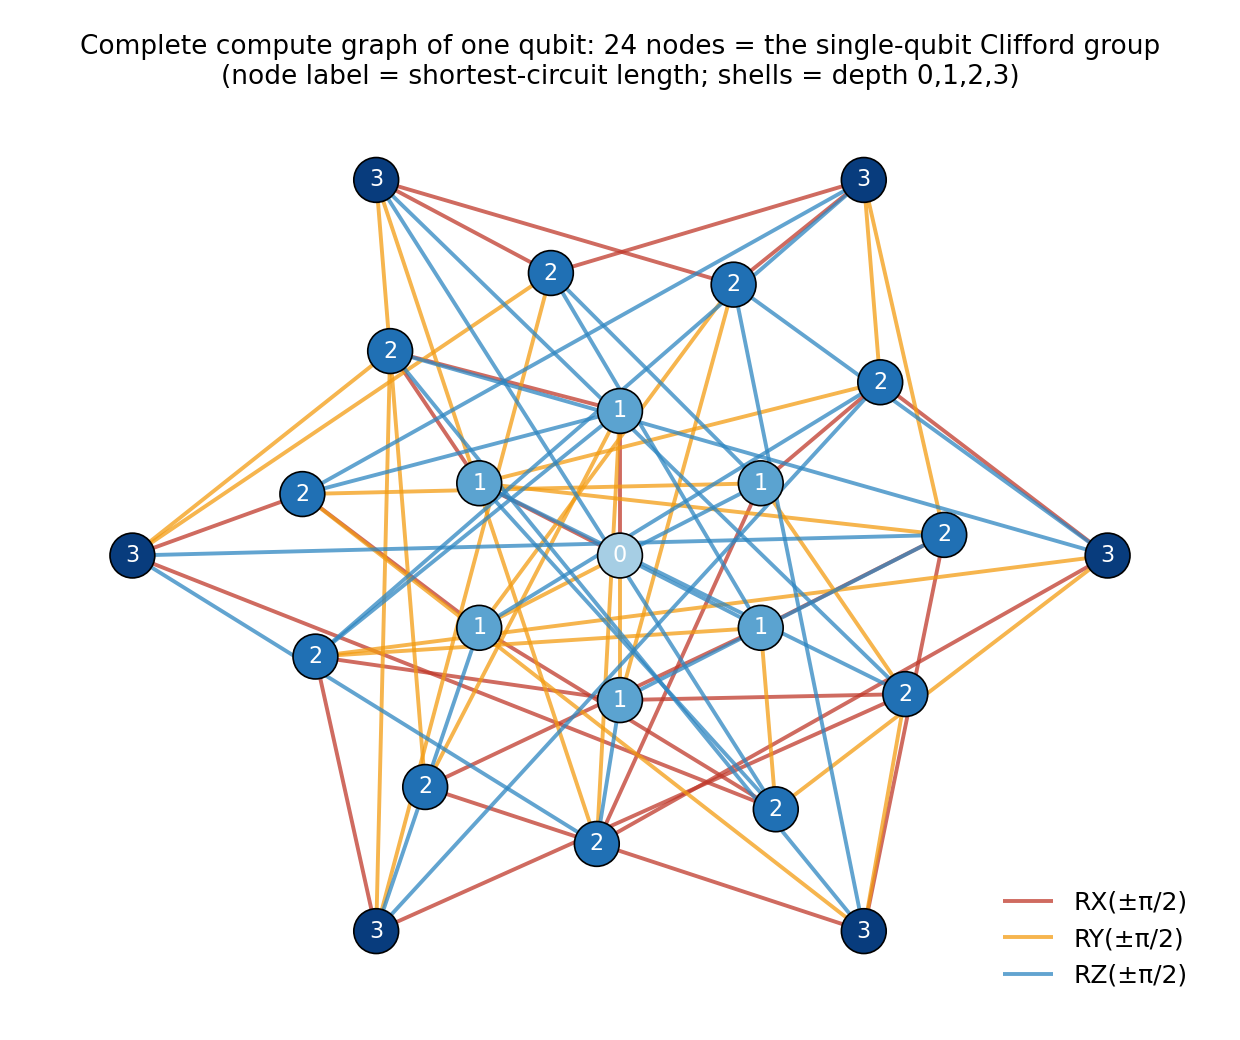
\includegraphics[width=0.78\linewidth]{figs/notes_1q_graph.png}\\
      {\scriptsize\color{muted}One qubit: the complete compute graph has exactly 24 nodes and diameter 3.}
    \end{column}
  \end{columns}
  \two{\takeaway{Optimality is no longer a vague question: each circuit has an exact shortest length, computable by search over one finite graph.}}
\end{frame}

\begin{frame}{Enumerating all 92.9 million 3-qubit Cliffords}
  \begin{columns}[T]
    \begin{column}{0.46\textwidth}
      \begin{itemize}\setlength{\itemsep}{0.5em}
        \item A Clifford mod phase = its signed \textbf{tableau}; for \(n\le3\) it packs into one 64-bit word.
        \item Gates act row-wise through lookup tables: each BFS level is a vectorised gather. Exact membership, no tolerance.
        \item Full BFS: 25\,min, \(\approx\)6\,GB, per alphabet.
      \end{itemize}
      \vspace{0.4em}
      \two{
      \centering\footnotesize\renewcommand{\arraystretch}{1.15}
      \begin{tabular}{@{}lrrr@{}}
        \toprule
        alphabet & \(n\) & diameter & mean optimal length\\\midrule
        ion trap & 2 & 10 & 5.89\\
        IBM-style & 2 & 11 & 6.92\\
        ion trap & 3 & \textbf{17} & \textbf{10.72}\\
        IBM-style & 3 & \textbf{19} & \textbf{12.34}\\\bottomrule
      \end{tabular}}
    \end{column}
    \begin{column}{0.52\textwidth}
      \two{
      \centering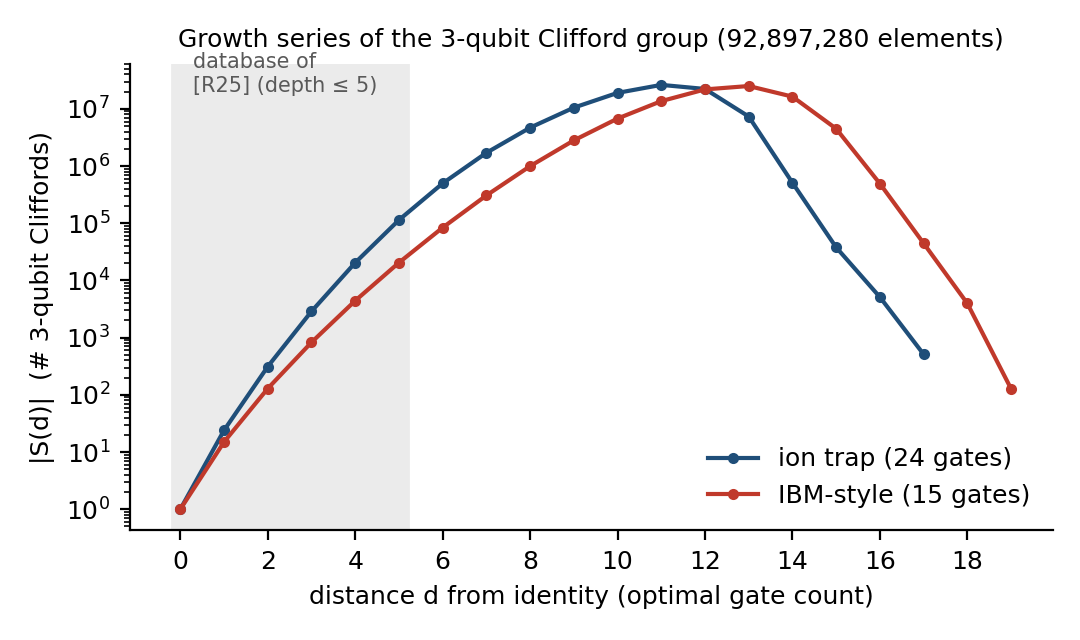
\includegraphics[width=\linewidth]{figs/ext_growth.png}\\
      {\scriptsize\color{muted}The paper's depth-5 database (shaded) covers 0.15\,\% of the group; almost all elements sit at distance 10--14.}}
    \end{column}
  \end{columns}
\end{frame}

\begin{frame}{How far from optimal is the paper's method?}
  \centering\footnotesize\renewcommand{\arraystretch}{1.25}
  \resizebox{\textwidth}{!}{\begin{tabular}{@{}lcccc@{}}
    \toprule
    3 qubits, 300 random gates, 20 circuits & \textbf{proven optimum} & paper's method (our port) & Qiskit 2.5 L3 & paper (1 circuit)\\\midrule
    ion trap & \textbf{10.4} & 47.1 & 127.2 & 45\\
    IBM-style & \textbf{12.2} & 36.8 & 104.0 & 72\\\bottomrule
  \end{tabular}}
  \vspace{1em}
  \two{
  \begin{columns}[T]
    \begin{column}{0.48\textwidth}
      \begin{alertblock}{The gap}
        The method's output is \textbf{4.5\(\times\)} (ion trap) and \textbf{3.0\(\times\)} (IBM-style) the optimum,
        on its own benchmark. Its showcase Fig.~4 output is 2\(\times\) optimal.
      \end{alertblock}
    \end{column}
    \begin{column}{0.48\textwidth}
      \begin{itemize}\setlength{\itemsep}{0.4em}\small
        \item Our port matches the paper's own single-circuit number (47.1 vs.\ 45), so this is the method, not the implementation.
        \item Beating Qiskit by 2.7\(\times\) looked impressive; another 4.5\(\times\) was available.
      \end{itemize}
    \end{column}
  \end{columns}}
\end{frame}

\begin{frame}{Exact windows close the gap}
  \begin{columns}[T]
    \begin{column}{0.52\textwidth}
      \centering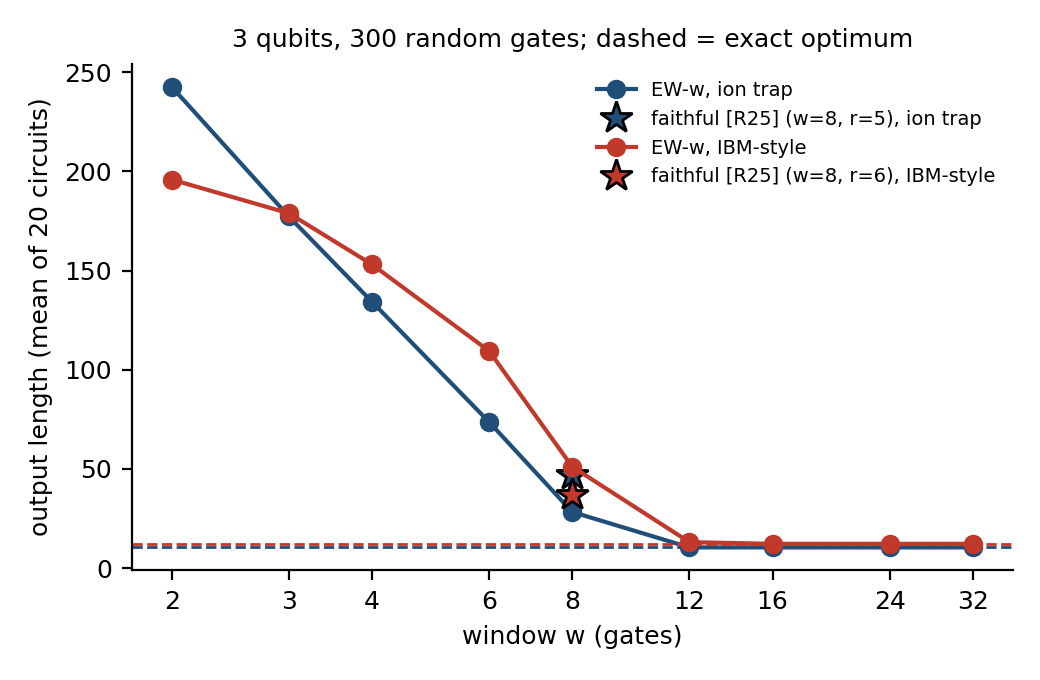
\includegraphics[width=\linewidth]{figs/ext_window.png}
    \end{column}
    \begin{column}{0.46\textwidth}
      \begin{itemize}\setlength{\itemsep}{0.5em}
        \item \textbf{Exact-window optimiser} EW-\(w\): replace every window of \(\le w\) gates on \(\le3\) wires by its \emph{proven} optimal word (table lookup).
      \end{itemize}
      \two{
      \begin{itemize}\setlength{\itemsep}{0.5em}
        \item Sharp transition: \(w\ge12\) (ion) / \(w\ge16\) (IBM-style) reaches the \textbf{proven optimum on all 40 circuits}.
        \item 0.1--0.2\,s per circuit, vs.\ 51\,s / 17\,s for the paper's method.
        \item Why so sharp? Once the circuit is shorter than the window, one more sweep is exact (the \emph{cascade}, Part IV).
      \end{itemize}}
    \end{column}
  \end{columns}
\end{frame}

\begin{frame}{What actually limits the original method: window or database?}
  \begin{columns}[T]
    \begin{column}{0.50\textwidth}
      \centering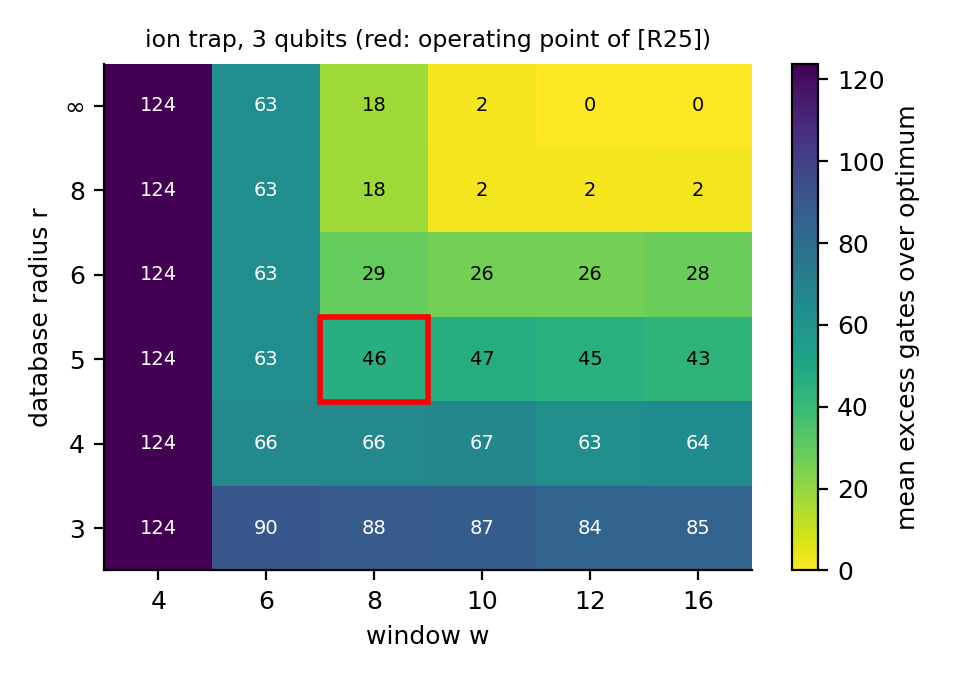
\includegraphics[width=0.95\linewidth]{figs/ext_grid.png}\\
      {\scriptsize\color{muted}Mean excess over the optimum (ion trap, 3 qubits) by window \(w\) and database radius \(r\). Red: the paper's \((8,5)\).}
    \end{column}
    \begin{column}{0.48\textwidth}
      \two{
      \begin{itemize}\setlength{\itemsep}{0.6em}
        \item Larger window at \(r=5\): excess 46 \(\to\) 43. Barely helps.
        \item Larger database at \(w=8\): excess 46 \(\to\) 18.
        \item \(w\ge12\) and \(r\ge8\): excess \(\le 2\).
      \end{itemize}
      \takeaway{The \textbf{database radius}, not the window or the search strategy, is the binding constraint. The theory predicts both are needed.}}
    \end{column}
  \end{columns}
\end{frame}

\begin{frame}{Four qubits: the journal benchmark}
  \centering\footnotesize\renewcommand{\arraystretch}{1.2}
  \resizebox{\textwidth}{!}{\begin{tabular}{@{}lccccccc@{}}
    \toprule
    4q, 300 gates, 100 circuits & lower bound & CW-sem & CW-24 & contiguous EW-16 & port & published & Qiskit L3\\\midrule
    ion trap: total & \(\ge\)11.1 & \good{45.6} & 56.7 & 110.3 & 78.8 & 111 & 164.9\\
    IBM-style: total & \(\ge\)12.9 & \good{49.3} & 59.1 & 130.9 & 76.0 & 107 & 140.9\\
    ion: RXX / IBM: CZ & -- & -- & 27.6 / 27.1 & 44.2 / 47.1 & 33.3 / 32.4 & 43 / 43 & 47.3 / 47.3\\\bottomrule
  \end{tabular}}
  \vspace{0.8em}
  \two{
  \begin{itemize}\setlength{\itemsep}{0.4em}\small
    \item Same exact 3-qubit oracle, different windows: contiguous windows (EW-16) are \emph{no better} than published;
          \textbf{DAG-convex windows} (CW-24) cut the published results by 49\,\% / 45\,\%; adaptive commutation-aware windows (CW-sem) go further.
    \item Two-qubit counts (27.6 RXX / 27.1 CZ) reach the journal's BQSKit numbers (28 / 37) without targeting them.
    \item No exact optimum at 4 qubits (\(|G|=1.2\times10^{13}\)), but a certified lower bound; the remaining gap is at most \(\approx4\times\).
  \end{itemize}}
\end{frame}

% ################################################################ PART IV
\partslide{IV}{Theory}{Local rewriting as rewriting on a Cayley graph: when is it exact, what can it never do, and what do random benchmarks measure?}

\begin{frame}{The model}
  \begin{columns}[T]
    \begin{column}{0.48\textwidth}
      \begin{itemize}\setlength{\itemsep}{0.5em}
        \item Alphabet \(\Gamma\), group \(G=\langle\Gamma\rangle\), word length \(|g|\), ball \(B(r)\), diameter \(D\).
        \item Compute graph of depth \(d\) \(=\) ball \(B(d)\) in \(\mathrm{Cay}(G,\Gamma)\); stored words are geodesics.
        \item Rewriting system \(\mathcal R(w,r)\): replace a factor of length \(\le w\) by an equivalent geodesic of length \(\le r\).
      \end{itemize}
    \end{column}
    \begin{column}{0.48\textwidth}
      \two{
      \begin{itemize}\setlength{\itemsep}{0.5em}
        \item Swapping commuting neighbours = moves in the \textbf{trace monoid}.
        \item Factors of trace-equivalent words = \textbf{convex} sets of the circuit DAG.
        \item So the paper's random commuting shuffles are a \emph{stochastic enumeration of convex windows}; we enumerate them directly.
        \item The paper's V2 operates at \((w,r)=(8,5)\).
      \end{itemize}}
    \end{column}
  \end{columns}
\end{frame}

\begin{frame}{Theorem 1: local = global above the diameter}
  \begin{block}{Exactness threshold}
    Let \(G\) be finite with diameter \(D\). If \(w\ge D+1\) and \(r\ge D\), every \((w,r)\)-reduced word is a geodesic.
  \end{block}
  \small\textit{Proof idea.} A reduced word longer than \(D\) would have a first factor of length \(D+1\), which is not geodesic and fits in the window. So the word has length \(\le D<w\), and then the whole word is one window.
  \vspace{0.6em}
  \two{
  \begin{columns}[T]
    \begin{column}{0.48\textwidth}
      \begin{block}{Cascade}
        If at any time the current length \(\ell \le w\), the next sweep returns a geodesic. Relevant window:
        \(w^\star=\min\{w:\ell(w)\le w\}\).
      \end{block}
    \end{column}
    \begin{column}{0.48\textwidth}
      \begin{itemize}\setlength{\itemsep}{0.3em}\small
        \item Measured \(w^\star\approx12\) (ion) / 16 (IBM-style) for 3 qubits, well below \(D+1=18\).
        \item The paper's \((8,5)\) is below both thresholds.
        \item Continuous gate sets: \(D=\infty\), no finite window is exact. Hence ground truth must come from the discrete case.
      \end{itemize}
    \end{column}
  \end{columns}}
\end{frame}

\begin{frame}{Theorem 2: gate-count parity}
  \begin{block}{Parity}
    (a) For \(n\le2\) the Cayley graph is \textbf{bipartite}: every equivalent rewrite removes an \emph{even} number of gates.\\
    (b) For \(n\ge3\), with any generating set containing square roots of each \(X_i\), \(Z_i\), it is \textbf{never} bipartite.
  \end{block}
  \small\textit{Proof idea.} Bipartite \(\iff\) a sign character \(\chi\) with \(\chi(\Gamma)=-1\). For \(n\ge3\), \(\chi\) kills the Paulis and factors through \(\mathrm{Sp}(2n,2)\), which is simple: \(\chi\equiv1\).
  \vspace{0.6em}
  \two{
  \begin{itemize}\setlength{\itemsep}{0.4em}
    \item Exhaustive search, 3 qubits: the shortest odd relation has length \(\rho=11\) (ion) / 9 (IBM-style).
          Changing parity needs a window of \(\ge6\) gates; smaller windows can never reach an optimum of the other parity.
    \item The paper's Fig.~4 shows a \(6\to3\) replacement on two qubits: \textbf{impossible} with the stated gate set.
  \end{itemize}}
\end{frame}

\begin{frame}{Theorem 3: random-circuit benchmarks measure a constant}
  \begin{columns}[T]
    \begin{column}{0.48\textwidth}
      \begin{block}{Benchmarks mix}
        A random word of length \(L\) is within \(\tfrac12\sqrt{|G|}\,\beta^L\) (total variation) of a uniform group element.
        So \(\mathbb E[\text{optimal length}]\to\) the mean distance in \(G\).
      \end{block}
      \vspace{0.3em}
      \small 2 qubits, ion trap: \(\beta=0.937\) (sparse diagonalisation).
    \end{column}
    \begin{column}{0.50\textwidth}
      \centering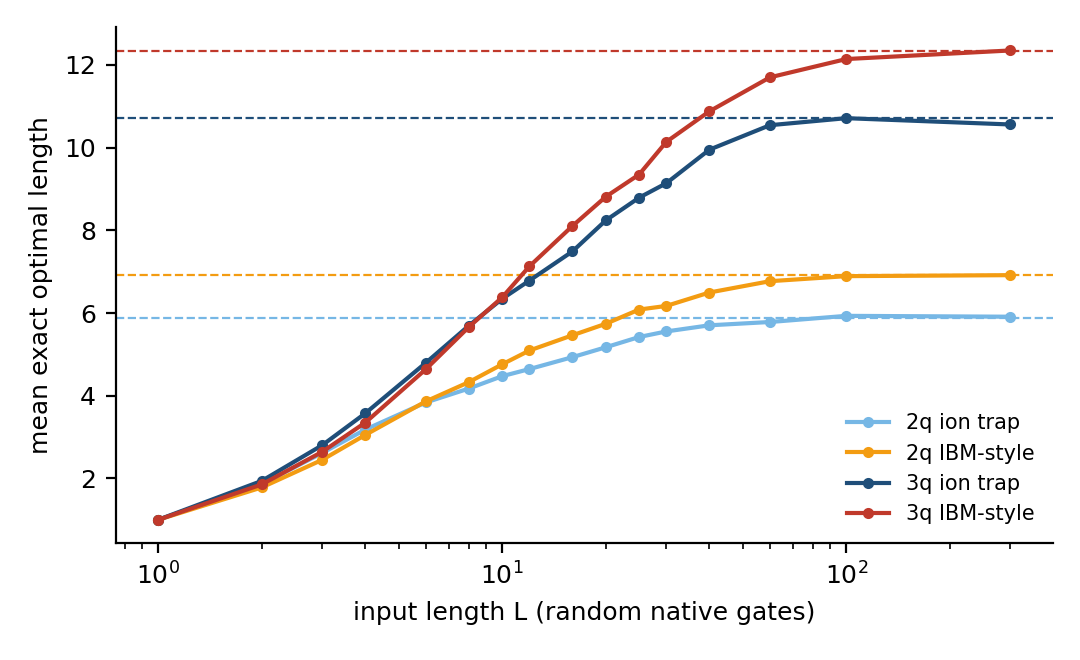
\includegraphics[width=\linewidth]{figs/ext_mixing.png}
    \end{column}
  \end{columns}
  \two{\takeaway{``Reduced from 300 to 45 gates'' mostly measures the input length. Beyond \(L\approx100\), every random 3-qubit ion circuit has optimum \(\approx10.7\) on average, whatever \(L\) is.}}
\end{frame}

\begin{frame}{Lower bounds for every method (4 qubits)}
  \begin{columns}[T]
    \begin{column}{0.48\textwidth}
      \begin{block}{Counting bound}
        \(\Pr[|g|\le d]\le|B(d)|/|G|\), and spheres are submultiplicative, \(|S(a+b)|\le|S(a)||S(b)|\).
        Exact spheres up to a small depth bound \(\mathbb E|g|\) from below for any optimiser.
      \end{block}
    \end{column}
    \begin{column}{0.48\textwidth}
      \two{
      \begin{itemize}\setlength{\itemsep}{0.5em}
        \item Check at \(n=3\): bound 7.9 vs.\ truth 10.72.
        \item \(n=4\) (\(1.2\times10^{13}\) elements), spheres to depth 6: \(\mathbb E|g|\ge\) \textbf{11.1} (ion) / \textbf{12.9} (IBM-style).
        \item Best achieved: 45.6 / 49.3. Closing that gap is an open problem the framework makes precise.
      \end{itemize}}
    \end{column}
  \end{columns}
\end{frame}

% ################################################################ PART V
\partslide{V}{A general optimiser}{Drop the Clifford crutch: continuous angles, connectivity, calibrated noise, and a precise notion of ``equivalent''.}

\begin{frame}{Why go beyond Clifford?}
  \begin{columns}[T]
    \begin{column}{0.48\textwidth}
      \textbf{The Clifford results don't transfer}
      \begin{itemize}\setlength{\itemsep}{0.4em}
        \item Real compilers emit \textbf{arbitrary angles} (\(R_z(\theta)\), MS\((\theta)\)): no finite group, no tables.
        \item Real chips have \textbf{connectivity} (heavy-hex) and per-gate \textbf{calibrated errors}.
        \item ``Up to global phase'' is \textbf{unsafe} once a block is controlled.
        \item Total gate count is the wrong objective when 2q gates dominate error.
      \end{itemize}
    \end{column}
    \begin{column}{0.48\textwidth}
      \two{
      \textbf{Design decisions}
      \begin{itemize}\setlength{\itemsep}{0.4em}
        \item \textbf{No} Clifford assumption in the method; Clifford tables only to \emph{evaluate}.
        \item Devices: IBM Heron (FakeTorino: \(R_z(\theta)\), \(\sqrt X\), \(X\), CZ, heavy-hex, calibrated) and a trapped-ion model
              (\(R_{x,y,z}(\theta)\), \(R_{XX}(\theta)\), all-to-all).
        \item Semantics: exact incl.\ phase, state/measurement-aware, approximate with tracked error.
        \item Objective: chosen by noisy simulation, not assumed.
      \end{itemize}}
    \end{column}
  \end{columns}
\end{frame}

\begin{frame}{One idea: equivalence = group action, key = canonical orbit}
  \footnotesize\renewcommand{\arraystretch}{1.1}
  \begin{tabularx}{\textwidth}{@{}>{\raggedright\arraybackslash}p{0.30\textwidth}>{\raggedright\arraybackslash}X>{\raggedright\arraybackslash}p{0.28\textwidth}@{}}
    \toprule
    \textbf{notion} & \(U \sim V\) \textbf{iff} & \textbf{canonical database key}\\
    \midrule
    exact & \(V = U\) & raw matrix\\
    up to phase (the paper) & \(V = e^{i\varphi} U\) & phase-normalised matrix\\
    input-aware (at start) & \(V|0\rangle = e^{i\varphi}U|0\rangle\) & phase-normalised \(U|0\rangle\)\\
        output-aware (before readout) & \(V = D\,U\), \(D\) diagonal & rows phase-normalised\\
    symmetry & \(V = P U P^{\dagger}\), \(P\) a chip symmetry & minimum over the orbit\\
    approximate & \(\lVert U - V\rVert \le \varepsilon\) & exact key + verified distance\\
    \bottomrule
  \end{tabularx}
  \vspace{0.6em}
  \uncover<2->{%
  \begin{block}{One engine, many semantics}
    The database stores 64-bit hashes of canonical forms: one lookup finds the whole class.
    New semantics = new key function. Every hit is re-verified numerically.
  \end{block}}
\end{frame}

\begin{frame}{Why the relaxed semantics are safe}
  \begin{block}{Proposition 1 (state- and measurement-aware rewriting)}
    Program: prepare \(|0^n\rangle\), run the circuit, measure all qubits. For a convex window \(S\) on wires \(W\):
    (a) if nothing precedes \(S\) on \(W\) and \(V|0_W\rangle = e^{i\varphi}U|0_W\rangle\), or
    (b) if nothing follows \(S\) on \(W\) and \(V = DU\) with \(D\) diagonal,
    then replacing \(U\) by \(V\) leaves the output distribution unchanged, and so does any sequence of such rewrites.
  \end{block}
  \small\textit{Why.} (a) the input is a product state; (b) \(|\langle x|D\psi\rangle|^2=|\langle x|\psi\rangle|^2\). The invariant is the output distribution.
  \vspace{0.5em}
  \two{
  \begin{block}{Proposition 2 (approximate rewriting)}
    If rewrite \(i\) has operator-norm error \(\varepsilon_i\), the final circuit is within \(\sum_i\varepsilon_i\) of the original (including phase in exact mode).
  \end{block}
  \small\textit{Why.} Telescoping, and \(\lVert A(X-Y)B\rVert=\lVert X-Y\rVert\) for unitary \(A,B\). The optimiser reports this bound with every circuit.}
\end{frame}

\begin{frame}{The engine}
  \begin{columns}[T]
    \begin{column}{0.52\textwidth}
      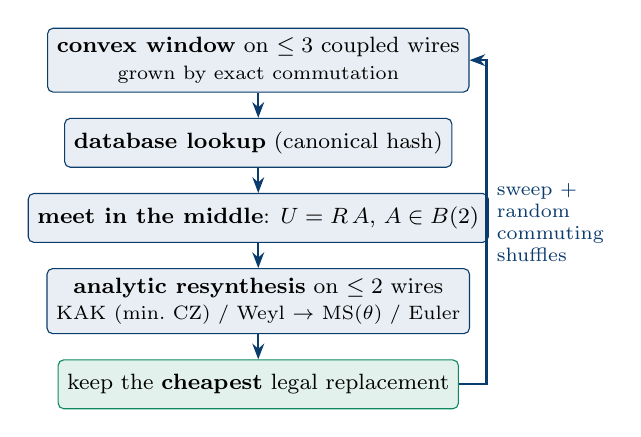
\begin{tikzpicture}[node distance=0.32cm, every node/.style={font=\footnotesize},
          box/.style={draw=ibar,fill=ifoot,rounded corners=2pt,minimum width=4.9cm,minimum height=0.62cm,align=center},
          arr/.style={-{Stealth[length=2mm]},ibar,thick}]
        \node[box] (w) {\textbf{convex window} on \(\le3\) coupled wires\\{\scriptsize grown by exact commutation}};
        \node[box,below=of w] (d) {\textbf{database lookup} (canonical hash)};
        \node[box,below=of d] (m) {\textbf{meet in the middle}: \(U=R\,A\), \(A\in B(2)\)};
        \node[box,below=of m] (r) {\textbf{analytic resynthesis} on \(\le2\) wires\\{\scriptsize KAK (min.\ CZ) / Weyl \(\to\) MS\((\theta)\) / Euler}};
        \node[box,below=of r,fill=igreen!12,draw=igreen] (a) {keep the \textbf{cheapest} legal replacement};
        \draw[arr] (w)--(d); \draw[arr] (d)--(m); \draw[arr] (m)--(r); \draw[arr] (r)--(a);
        \draw[arr] (a.east) -- ++(0.35,0) |- node[pos=0.25,right,align=left,font=\scriptsize\color{muted}]{sweep +\\ random\\ commuting\\ shuffles} (w.east);
      \end{tikzpicture}
    \end{column}
    \begin{column}{0.46\textwidth}
      \two{
      \centering\footnotesize\renewcommand{\arraystretch}{1.12}
      \resizebox{\linewidth}{!}{\begin{tabular}{@{}llrr@{}}
        \toprule
        \textbf{device, topology} & \textbf{notion} & \textbf{classes} & \textbf{depth}\\
        \midrule
        Heron, line & phase & 6.31\,M & 9\\
                    & output-aware & 0.34\,M & 10\\
                    & input-aware & 1.41\,M & 14\\
        ion, triangle & phase & 28.4\,M & 6\\
                      & output-aware & 7.36\,M & 6\\
                      & input-aware & 31.6\,M & 7\\
        paper ion alphabet & phase & 2.93\,M & 9\\
        paper IBM alphabet & phase & 1.84\,M & 10\\
        \bottomrule
      \end{tabular}}\\[0.3em]
      {\scriptsize\color{muted}Grid: angles \(\pm\frac\pi4,\pm\frac\pi2,\pi\); 23 (Heron) / 57 (ion) local gates. Build: 18\,s -- 38\,min. Deepest level stored as keys only.}}
    \end{column}
  \end{columns}
\end{frame}

\begin{frame}{Global phase and cost: the details that matter}
  \begin{columns}[T]
    \begin{column}{0.48\textwidth}
      \textbf{Exact including global phase}
      \begin{itemize}\setlength{\itemsep}{0.4em}
        \item Inside windows, match up to phase and record each phase.
        \item Native gates reach only a \emph{discrete} set of phases: multiples of \(\pi/4\) (Heron), \(\pi/2\) (ion). Snap, or reject.
        \item Repair once at the end with the cheapest gadget; on ions absorb \(\pm i\) into an existing MS gate:
              \(R_{XX}(\theta\pm\pi)\,R_x(\pi)^{\otimes 2} = \pm i\,R_{XX}(\theta)\).
        \item Never return a costlier circuit than the input.
      \end{itemize}
    \end{column}
    \begin{column}{0.48\textwidth}
      \two{
      \textbf{Three candidate objectives}
      \[
        c_{\rm count}=1,\qquad c_{w2}=\begin{cases}10&\text{2q}\\1&\text{1q}\end{cases}
      \]
      \[
        c_{\rm cal}(g)=-\log\bigl(1-e(g)\bigr)
      \]
      \begin{itemize}\setlength{\itemsep}{0.4em}
        \item \(e^{-c_{\rm cal}}\) = estimated success probability (ESP): minimising \(c_{\rm cal}\) maximises ESP.
        \item \(e(g)\) from FakeTorino calibration per qubit / pair; ion model \(3\cdot10^{-5}\) / \(10^{-3}\); \(R_z\) virtual.
        \item Which one wins is decided by noisy simulation (Part VI).
      \end{itemize}}
    \end{column}
  \end{columns}
\end{frame}

% ################################################################ PART VI
\partslide{VI}{Results}{First the paper's own benchmarks against ground truth, then 60 standard circuits on hardware models.}

\begin{frame}{Result 1: the paper's benchmarks, without Clifford knowledge}
  \begin{columns}[c]
    \begin{column}{0.60\textwidth}
      \centering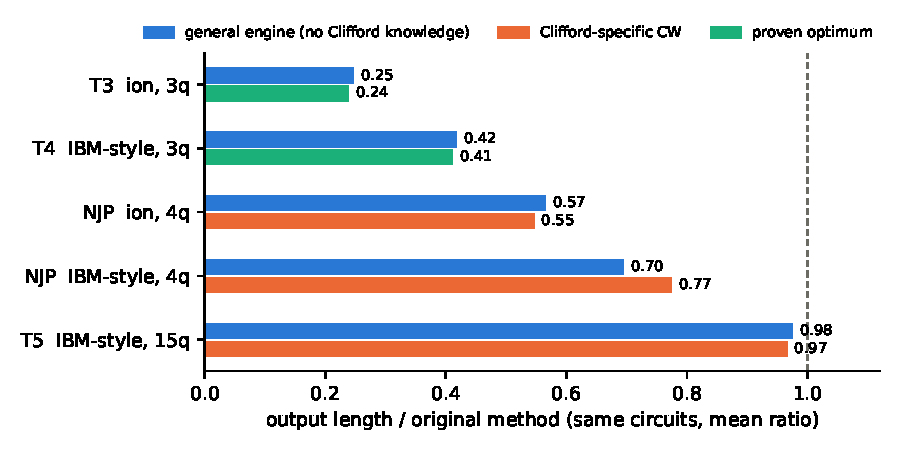
\includegraphics[width=\linewidth]{figs/gen_paper_bench.pdf}\\
      {\scriptsize\color{muted}Output length / paper's method, same circuits and seeds. Paper semantics: up to phase, gate count, \(\pm\frac\pi2\) alphabets.}
    \end{column}
    \begin{column}{0.38\textwidth}
      \two{
      \begin{itemize}\setlength{\itemsep}{0.5em}
        \item \textbf{3 qubits}: proven optimum on \textbf{17/20} (ion) and \textbf{18/20} (IBM-style); mean 10.8 vs.\ optimum 10.4.
        \item \textbf{4 qubits}: on par with the Clifford-specific optimiser (46.1 vs.\ 45.6; 51.4 vs.\ 49.3).
        \item \textbf{15 qubits}: all methods within 4\,\%.
        \item 3--9\,s per circuit; all 250 outputs verified and native.
      \end{itemize}}
    \end{column}
  \end{columns}
  \two{\takeaway{Knowing the group structure is not what makes the difference; large databases and convex windows are.}}
\end{frame}

\begin{frame}{Result 2: standard suites on hardware models --- setup}
  \begin{columns}[T]
    \begin{column}{0.49\textwidth}
      \textbf{Circuits} (60 per device, 2--12 qubits, \(\le\)1,008 gates)
      \begin{itemize}\setlength{\itemsep}{0.3em}
        \item Nam/VOQC arithmetic: Toffoli/Barenco ladders, adders, modular multiplication, \(\mathrm{GF}(2^4)\) multiplier, product formulas, QFT8
        \item QASMBench small/medium (4 with classical feed-forward and 4 unparsable skipped)
        \item QFT, QAOA, Heisenberg Trotter, EfficientSU2, Steane encoder
        \item Random non-Clifford circuits
      \end{itemize}
    \end{column}
    \begin{column}{0.49\textwidth}
      \two{
      \textbf{Pipelines} (same native set, coupling map, seed)
      \begin{itemize}\setlength{\itemsep}{0.3em}
        \item Qiskit transpile, levels 1 and 3
        \item TKET \texttt{FullPeepholeOptimise} on L1 + rebase
        \item ours on L1 output; \textbf{ours on L3 output}
      \end{itemize}
      \vspace{0.5em}
      \textbf{Metrics}: 2q count, total, depth, ESP, noisy-simulation TVD (\(\le 8\) active qubits); every output verified, native, coupled.}
    \end{column}
  \end{columns}
\end{frame}

\begin{frame}{Result 2: relative to Qiskit level 3}
  \centering\footnotesize\renewcommand{\arraystretch}{1.22}
  \begin{tabular}{@{}l ccc c cc@{}}
    \toprule
    & \multicolumn{3}{c}{\textbf{IBM Heron} (58 circuits)} && \multicolumn{2}{c}{\textbf{trapped ion} (58 circuits)}\\
    \cmidrule{2-4}\cmidrule{6-7}
    \textbf{pipeline} & 2q gates & all gates & ESP && 2q gates & all gates\\
    \midrule
    TKET                                & \(\times\)1.02 & \(\times\)1.71 & \(\times\)1.16 && \(\times\)1.27 & \(\times\)1.79\\
    ours, exact, from Qiskit L1         & \(\times\)1.00 & \good{\(\times\)0.84} & \good{\(\times\)1.21} && \good{\(\times\)0.95} & \good{\(\times\)0.76}\\
    ours, exact, from Qiskit L3         & \good{\(\times\)0.98} & \good{\(\times\)0.87} & \(\times\)1.03 && \(\times\)1.00 & \(\times\)1.00\\
    ours, approximate (\(\varepsilon=10^{-3}\)), from L1 & \(\times\)1.01 & \good{\(\times\)0.84} & \good{\(\times\)1.21} && \good{\(\times\)0.95} & \good{\(\times\)0.75}\\
    ours, state/measurement-aware       & \good{\(\times\)0.77} & \good{\(\times\)0.61} & \good{\(\times\)1.28} && \good{\(\times\)0.62} & \good{\(\times\)0.50}\\
    \bottomrule
  \end{tabular}
  \vspace{0.6em}
  \two{
  \begin{itemize}\setlength{\itemsep}{0.3em}\small
    \item \textbf{Stacked on L3}: never more 2q gates (Heron 9 better / 49 equal; ion 1 / 57) and never lower ESP, on either device.
    \item TKET keeps 2q counts close to L3 but needs 1.7--1.8\(\times\) the gates after rebasing.
    \item Ion ESPs differ by \(<1\,\%\) across pipelines (MS error \(10^{-3}\)), so they are omitted.
  \end{itemize}}
  \src{Ratios of summed counts; ESP: geometric mean of per-circuit ratios. Nam pf1\_10/pf2\_10 excluded: Qiskit L3 drops their \(10^{-7}\)\,rad rotations (approximate, not exact).}
\end{frame}

\begin{frame}{Where do the gains come from? (honest accounting)}
  \begin{columns}[T]
    \begin{column}{0.48\textwidth}
      \textbf{Stacked on L3, summed over 58 circuits}\\[0.3em]
      \footnotesize\renewcommand{\arraystretch}{1.2}
      \begin{tabular}{@{}lrr@{}}
        \toprule
        & Qiskit L3 & + ours\\\midrule
        Heron \(\sqrt X/X\) pulses & 7,218 & 6,139\\
        Heron \(R_z\) (virtual) & 5,297 & 4,436\\
        Heron CZ & 2,889 & 2,830\\\midrule
        ion \(R_x/R_y\) pulses & 3,824 & 2,422\\
        ion \(R_z\) (virtual) & 2,223 & \bad{3,622}\\
        ion MS & 1,378 & 1,376\\\bottomrule
      \end{tabular}
    \end{column}
    \begin{column}{0.48\textwidth}
      \two{
      \begin{itemize}\setlength{\itemsep}{0.5em}\small
        \item Heron: savings split between pulses and \(R_z\); a few CZ.
        \item Ion: the calibrated objective \emph{trades} pulses for free \(R_z\). The total rises on 28/58 circuits, by design.
              ``Never worse'' holds for the objective, 2q count and ESP, \textbf{not} for the total.
        \item ESP \(\times\)1.21 from L1 decomposes as \(\times\)1.11 (Qiskit's L1 layout already beats its L3 layout) \(\times\) \(\times\)1.09 (our rewriting).
              We never change the layout.
      \end{itemize}}
    \end{column}
  \end{columns}
\end{frame}

\begin{frame}{Which objective? Let noisy simulation decide}
  \begin{columns}[c]
    \begin{column}{0.48\textwidth}
      \centering\renewcommand{\arraystretch}{1.25}\small
      \resizebox{\linewidth}{!}{\begin{tabular}{@{}lcc@{}}
        \toprule
        & \multicolumn{2}{c}{\textbf{mean TVD} (49 circuits)}\\
        \textbf{pipeline / objective} & Heron & ion\\
        \midrule
        Qiskit L1                  & 0.115 & 0.0157\\
        Qiskit L3                  & 0.137 & 0.0091\\
        ours, total count          & 0.096 & 0.0092\\
        ours, 2q-weighted          & \good{0.088} & \good{0.0084}\\
        ours, calibrated \(-\log F\) & \good{0.088} & \good{0.0084}\\
        \bottomrule
      \end{tabular}}\\[0.4em]
      {\scriptsize\color{muted}Exact density-matrix probabilities (no shot noise). Heron: FakeTorino gate errors of the actual qubits. Ion: depolarising model.}
    \end{column}
    \begin{column}{0.50\textwidth}
      \two{
      \centering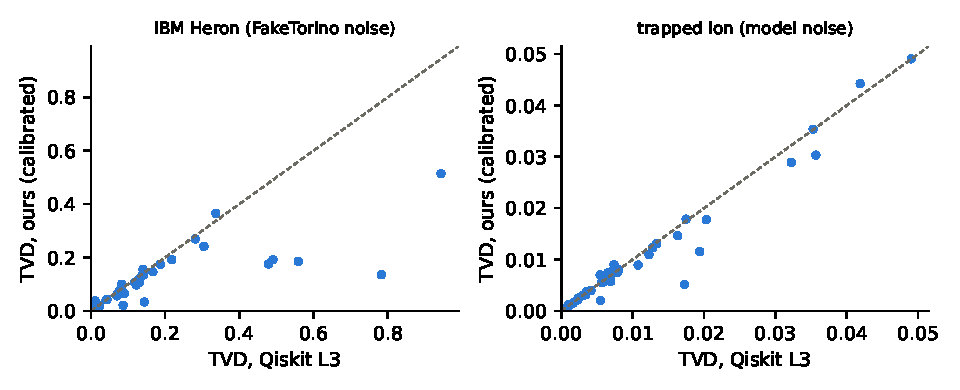
\includegraphics[width=\linewidth]{figs/gen_tvd.pdf}\\
      \begin{itemize}\setlength{\itemsep}{0.3em}\small
        \item Calibrated beats L3 on \textbf{39/49} (Heron) and 29/49 (ion) circuits.
        \item Calibrated \(\approx\) 2q-weighted \(>\) count \(\Rightarrow\) calibrated is the default; 2q-weighted is a good proxy without calibration data.
      \end{itemize}}
    \end{column}
  \end{columns}
\end{frame}

\begin{frame}{The other semantics: state-aware and approximate}
  \begin{columns}[T]
    \begin{column}{0.48\textwidth}
      \begin{block}{State/measurement-aware}
        \begin{itemize}\setlength{\itemsep}{0.3em}
          \item Largest gains: 2q gates \(\times\)0.77 (Heron) / \(\times\)0.62 (ion) relative to L3.
          \item Output distributions agree to \(6\cdot10^{-12}\).
          \item Valid only for a complete program: \(|0\cdots0\rangle\) in, full measurement out.
        \end{itemize}
      \end{block}
      \two{\small\color{iorange}Caveat: 5 (Heron) / 7 (ion) circuits are reversible logic on \(|0\cdots0\rangle\) with a fixed basis-state output; they reduce to the
      empty circuit. Read this mode per circuit, not as an average.}
    \end{column}
    \begin{column}{0.48\textwidth}
      \two{
      \begin{block}{Approximate (\(\varepsilon=10^{-3}\) per replacement)}
        \begin{itemize}\setlength{\itemsep}{0.3em}
          \item Almost no gain over exact on these suites: few near-identity blocks.
          \item Measured error always inside the tracked bound (max \(6.4\cdot10^{-4}\)).
          \item Exception: Nam pf2\_10 (rotations \(\sim10^{-7}\)\,rad): 1,088 \(\to\) 529 gates, error \(1.3\cdot10^{-4}\) \(\le\) bound \(7.1\cdot10^{-4}\).
        \end{itemize}
      \end{block}}
    \end{column}
  \end{columns}
\end{frame}

\begin{frame}{Verification: every number on these slides is checked}
  \begin{columns}[T]
    \begin{column}{0.48\textwidth}
      \begin{itemize}\setlength{\itemsep}{0.5em}
        \item \textbf{Exact mode}: \(\lVert (U-V)\psi\rVert\) on random states, statevector on the active qubits: \(\le 8.2\cdot10^{-11}\).
        \item \textbf{State-aware}: TVD of output distributions: \(\le 6\cdot10^{-12}\).
        \item \textbf{Approximate}: measured error \(\le\) tracked bound, all runs.
        \item \textbf{Legality}: native gates only, 2q gates only on working couplers.
      \end{itemize}
    \end{column}
    \begin{column}{0.48\textwidth}
      \two{
      \begin{itemize}\setlength{\itemsep}{0.5em}
        \item \textbf{Coverage}: 250/250 paper-benchmark outputs, 720/720 hardware-suite outputs.
        \item Nam pf2\_10 on Heron is routed over 20 physical qubits, beyond the main run's 16-qubit cap: re-run and verified separately (same totals).
        \item FakeTorino has 11 dead couplers (error 1.0); removed for \emph{all} pipelines after a first run put Qiskit L3 on them (ESP \(\sim10^{-22}\)).
      \end{itemize}}
    \end{column}
  \end{columns}
\end{frame}

% ################################################################ PART VII
\partslide{VII}{Wrap-up}{Lessons, limitations, critique of the original paper, and next steps.}

\begin{frame}{Lesson: ``exact'' is easy to get subtly wrong}
  Found on Nam \texttt{pf1\_10}/\texttt{pf2\_10} (rotations of \(\sim10^{-7}\)\,rad): outputs first verified only to \(10^{-6}\).
  \vspace{0.6em}
  \begin{columns}[T]
    \begin{column}{0.49\textwidth}
      \begin{alertblock}{Pitfalls}
        \begin{itemize}
          \item \texttt{np.allclose} has a default \emph{relative} tolerance \(10^{-5}\): near-commuting gates were swapped.
          \item \(|\mathrm{tr}(U^\dagger V)|/d \approx 1\) is \emph{quadratic} in the error: accepts \(\lVert U-V\rVert \sim 10^{-4}\).
          \item Native gates reach only a \emph{discrete} set of global phases.
        \end{itemize}
      \end{alertblock}
    \end{column}
    \begin{column}{0.49\textwidth}
      \two{
      \begin{exampleblock}{Fixes}
        \begin{itemize}
          \item Linear operator-distance tests, one tolerance \(10^{-10}\), \texttt{rtol=0}.
          \item Replacement phases snapped to the reachable set; residuals rejected or charged to \(\varepsilon\).
          \item Ion: \(\pm i\) absorbed into an existing MS gate.
        \end{itemize}
      \end{exampleblock}}
    \end{column}
  \end{columns}
  \two{\takeaway{\texttt{pf1\_10} now verifies to \(5\cdot10^{-13}\) (was \(1.8\cdot10^{-7}\)). The original paper uses three different tolerances up to \(10^{-3}\).}}
\end{frame}

\begin{frame}{Limitations of my work}
  \begin{columns}[T]
    \begin{column}{0.48\textwidth}
      \begin{itemize}\setlength{\itemsep}{0.6em}
        \item \textbf{Noise models, not hardware.} ESP and TVD from calibration snapshots; gate errors only (no readout, idle, crosstalk). Ion parameters are assumptions.
        \item \textbf{Global phase is not free for us.} Strict mode costs 240 single-qubit gates over the Heron suite; with phase as metadata (as Qiskit/TKET do), all gates \(\times\)0.838 \(\to\) \(\times\)0.825.
      \end{itemize}
    \end{column}
    \begin{column}{0.48\textwidth}
      \two{
      \begin{itemize}\setlength{\itemsep}{0.6em}
        \item \textbf{Baselines.} No BQSKit (not installable here), no Quartz/QUESO; one seed for Qiskit and TKET.
        \item \textbf{Local only.} Layout and routing are Qiskit's; windows \(\le3\) qubits; single-threaded Python (median 10\,s, max 180\,s per circuit vs.\ \(<\)1\,s for Qiskit).
        \item \textbf{Scope.} Circuits up to \(\sim\)1,000 gates; no mid-circuit measurement / feed-forward.
      \end{itemize}}
    \end{column}
  \end{columns}
\end{frame}

\begin{frame}{Weaknesses of the original paper}
  \begin{columns}[T]
    \begin{column}{0.48\textwidth}
      \begin{enumerate}\setlength{\itemsep}{0.4em}\small
        \item \textbf{Missing structure}: Clifford gate sets, but no tableaux, no exact keys; floating-point lookup with three tolerances; a classifier to speed up an avoidable \(O(N)\) scan.
        \item \textbf{No notion of optimality}: only compared with Qiskit; 4.5\(\times\) from an optimum computable in minutes.
        \item \textbf{Equivalence}: up-to-phase only, unsound under control; no state/measurement context; no error tracking.
        \item \textbf{Hardware model}: discrete angles, all-to-all, total count. Matches neither IBM nor ion hardware.
      \end{enumerate}
    \end{column}
    \begin{column}{0.48\textwidth}
      \two{
      \begin{enumerate}\setcounter{enumi}{4}\setlength{\itemsep}{0.4em}\small
        \item \textbf{Evaluation}: random benchmarks mix, so ``from 300 gates'' measures input length; one circuit per table; MATLAB vs.\ compiled timings.
        \item \textbf{Search}: contiguous windows, random swaps, no convergence criterion; radius 5 is the binding limit.
        \item \textbf{V3}: unreported features/threshold; 30\,\% recall at default.
        \item \textbf{Hardware evidence}: one 2-qubit circuit, no error bars; vanishes at Qiskit level 3.
        \item \textbf{Reproducibility}: only V2 released, with visible bugs; database for Tables III--V unstated.
      \end{enumerate}}
    \end{column}
  \end{columns}
\end{frame}

\begin{frame}{Summary}
  \begin{columns}[T]
    \begin{column}{0.48\textwidth}
      \begin{block}{About the paper}
        \begin{itemize}\setlength{\itemsep}{0.3em}
          \item Reproduces, with qualifications on database, forest threshold, baselines and transpiler level.
          \item Its gates are Clifford: exact optima show it is 3--4.5\(\times\) from optimal.
          \item Theory explains why: radius 5 and window 8 sit below the exactness threshold; random benchmarks measure a constant.
        \end{itemize}
      \end{block}
    \end{column}
    \begin{column}{0.48\textwidth}
      \two{
      \begin{exampleblock}{About the extension}
        \begin{itemize}\setlength{\itemsep}{0.3em}
          \item A general optimiser built on ``equivalence = group action'', with soundness and error bounds.
          \item Proven optimum on 35/40 of the paper's 3-qubit circuits without Clifford knowledge.
          \item On 58 real algorithms, stacked on Qiskit L3: never more 2q gates, never lower ESP, \(-13\,\%\) gates on Heron; lowest noisy error with the calibrated objective.
        \end{itemize}
      \end{exampleblock}}
    \end{column}
  \end{columns}
\end{frame}

\begin{frame}{Next steps, and questions for you}
  \begin{columns}[T]
    \begin{column}{0.48\textwidth}
      \textbf{Next steps}
      \begin{enumerate}\setlength{\itemsep}{0.4em}\small
        \item Layout-aware rewriting with calibrated costs (the biggest remaining lever on Heron).
        \item Cheaper exact phase repair on Heron.
        \item 4-qubit windows via symmetry reduction, or a learned admissible A\(^\ast\) heuristic trained on exact tables.
        \item Ground truth beyond Clifford: exact Clifford+T normal forms for small \(T\)-counts.
        \item BQSKit / Quartz baselines; real-hardware runs with error bars.
      \end{enumerate}
    \end{column}
    \begin{column}{0.48\textwidth}
      \two{
      \textbf{Where I'd like your input}
      \begin{enumerate}\setlength{\itemsep}{0.4em}\small
        \item Is the target a short note on the reproduction + optimality gap, or a full paper on the general framework?
        \item Is real-hardware access available for an error-barred experiment?
        \item Which venue fits: quantum-computing (theory + benchmarks) or a compiler venue?
        \item Should we contact the authors about the unstated database and the code bugs?
      \end{enumerate}}
    \end{column}
  \end{columns}
\end{frame}

\begin{frame}{Deliverables}
  \small\renewcommand{\arraystretch}{1.25}
  \begin{tabularx}{\textwidth}{@{}p{0.42\textwidth}X@{}}
    \toprule
    \textbf{What} & \textbf{Where}\\\midrule
    Study notes (read instead of the paper) & \texttt{manuscripts/notes/notes.pdf}\\
    Reproduction report (every table and figure) & \texttt{manuscripts/reproduction/reproduction\_report.pdf}\\
    Extension paper (12 pages) & \texttt{manuscripts/extension/extension\_paper.pdf}\\
    Python port, exact Clifford engine, general optimiser & \texttt{qcr/}\\
    Experiment scripts and raw results & \texttt{experiments/}, \texttt{results/}\\
    This talk & \texttt{manuscripts/talk/talk.pdf}\\\bottomrule
  \end{tabularx}
  \vfill
  \centering{\Large\bfseries\color{ibar} Thank you}
\end{frame}

% ================================================================ backup
\appendix
\section{Backup}
{\setbeamertemplate{footline}{}
\begin{frame}[plain]
  \begin{tikzpicture}[remember picture,overlay]
    \fill[ibar] (current page.south west) rectangle (current page.north east);
    \node[text=white,font=\Huge\bfseries] at (current page.center) {Backup};
  \end{tikzpicture}
\end{frame}}

\begin{frame}{Backup: paper-benchmark numbers (mean total gate count)}
  \centering\renewcommand{\arraystretch}{1.25}
  \resizebox{\textwidth}{!}{\begin{tabular}{@{}lrrrrr@{}}
    \toprule
    \textbf{set} & \textbf{Qiskit L3} & \textbf{paper's method} & \textbf{Clifford CW-sem} & \textbf{optimum / bound} & \textbf{general}\\
    \midrule
    T3 (ion, 3q, 20)          & 127.2 & 47.1  & --    & 10.4 & \good{10.8}\\
    T4 (IBM-style, 3q, 20)    & 104.0 & 36.8  & --    & 12.2 & \good{12.5}\\
    journal ion (4q, 100)     & 164.9* & 78.8* & 45.6  & \(\ge\)11.1 & \good{46.1}\\
    journal IBM-style (4q, 100) & 140.9* & 76.0* & 49.3  & \(\ge\)12.9 & \good{51.4}\\
    T5 (IBM-style, 15q, 10)   & 332.1 & 335.9 & 324.6 & --   & \good{327.7}\\
    \bottomrule
  \end{tabular}}\\[0.6em]
  {\footnotesize\color{muted}*first 30 circuits. General engine: up-to-phase semantics (as in the paper), total count, discrete \(\pm\pi/2\) alphabets, all-to-all.}
\end{frame}

\begin{frame}{Backup: minimal entangling-gate counts, 3 qubits}
  \centering\renewcommand{\arraystretch}{1.25}
  \resizebox{\textwidth}{!}{\begin{tabular}{@{}lrrrrrrr@{}}
    \toprule
    entangling gates & 0 & 1 & 2 & 3 & 4 & 5 & 6\\\midrule
    3-qubit Cliffords & 13,824 & 373,248 & 5,971,968 & 38,486,016 & 42,052,608 & 5,971,968 & 27,648\\\bottomrule
  \end{tabular}}\\[0.8em]
  {\small Mean 3.51, maximum 6. Identical for both alphabets (\(R_{XX}(\frac\pi2)\) and CZ are locally equivalent).
   For 2 qubits: 576 / 5,184 / 5,184 / 576 for 0--3, the known CNOT-count distribution.}
\end{frame}

\begin{frame}{Backup: worked examples from the reproduction}
  \begin{itemize}\setlength{\itemsep}{0.6em}
    \item \textbf{Fig.~1}: the 8-gate and 4-gate Bell circuits both equal CNOT\,(\(H\otimes I\)) to \(10^{-13}\); no 3-gate circuit exists.
    \item \textbf{Fig.~4 analogue} (2 qubits, 40 gates): \(40\to34\to26\to24\to20\to18\to16\to8\to4\); every step removes an even number of gates (parity theorem).
          The paper's final circuit contains an inverse pair; the optimum is 2.
    \item \textbf{Fig.~5 analogue} (3 qubits, 200 gates): \(200\to36\) in 31 replacements.
    \item \textbf{Authors' demo circuit} (5 qubits, 300 gates): authors 140; our port 140 (132--148) with the demo database, 115 (112--117) with the 24-op depth-5 database.
  \end{itemize}
\end{frame}

\end{document}
